% =====================================================================
% Amdox Technologies — AI-Powered Cloud ERP Suite
% Project Report (AMX-ERP-2026-04) — submission deliverable #1
% Build: latexmk -pdf Pawan_AMX_ERP_AmdoxTechnologies_April2026.tex
% =====================================================================
\documentclass[11pt,a4paper]{article}

% ---------- Layout & typography ----------
\usepackage[a4paper,top=2.2cm,bottom=2.4cm,left=2.2cm,right=2.2cm]{geometry}
\usepackage[T1]{fontenc}
\usepackage[utf8]{inputenc}
\usepackage{lmodern}
\usepackage{microtype}
\setlength{\emergencystretch}{3em}
\usepackage{parskip}
\usepackage{setspace}

% ---------- Colour & tables ----------
\usepackage[table]{xcolor}
\definecolor{amdoxnavy}{HTML}{0F2A4A}
\definecolor{amdoxblue}{HTML}{1F6FB2}
\definecolor{amdoxlight}{HTML}{EAF1F8}
\definecolor{okgreen}{HTML}{1A7A3C}
\definecolor{warnamber}{HTML}{B36B00}
\definecolor{gapred}{HTML}{A93226}
\usepackage{booktabs}
\usepackage{tabularx}
\usepackage{array}
\usepackage{multirow}
\usepackage{longtable}

% ---------- Graphics ----------
\usepackage{graphicx}
\graphicspath{{images/}}
\usepackage{tikz}
\usetikzlibrary{positioning,arrows.meta,shapes.geometric,fit,calc}

% ---------- Section styling ----------
\usepackage{titlesec}
\titleformat{\section}
  {\Large\bfseries\color{amdoxnavy}}
  {\thesection}{0.8em}{}[\vspace{2pt}{\color{amdoxblue}\titlerule[1.1pt]}]
\titleformat{\subsection}
  {\large\bfseries\color{amdoxnavy}}
  {\thesubsection}{0.7em}{}
\titleformat{\subsubsection}
  {\normalsize\bfseries\color{amdoxblue}}
  {\thesubsubsection}{0.6em}{}
\titlespacing{\section}{0pt}{14pt plus 3pt}{8pt}
\titlespacing{\subsection}{0pt}{10pt plus 2pt}{4pt}
\titlespacing{\subsubsection}{0pt}{8pt plus 2pt}{3pt}

% ---------- Header / footer ----------
\usepackage{fancyhdr}
\pagestyle{fancy}
\fancyhf{}
\fancyhead[L]{\small\color{amdoxnavy}\textbf{AMDOX TECHNOLOGIES}}
\fancyhead[R]{\small\color{gray}AI-Powered Cloud ERP Suite \;|\; AMX-ERP-2026-04}
\fancyfoot[L]{\small\color{gray}AMX-ERP-2026-04 \;|\; Project Report}
\fancyfoot[R]{\small\color{gray}Page \thepage}
\renewcommand{\headrulewidth}{0.6pt}
\renewcommand{\headrule}{\color{amdoxblue}\hrule width\headwidth height 0.6pt}

% ---------- Math & symbols ----------
\usepackage{amsmath}
\usepackage{amssymb}
\usepackage{textcomp}  % \textrightarrow, \textbullet, etc.

% ---------- Lists ----------
\usepackage{enumitem}
\setlist{nosep,leftmargin=1.4em}
\usepackage{float}

% ---------- Hyperlinks (load last) ----------
\usepackage[colorlinks=true,linkcolor=amdoxnavy,urlcolor=amdoxblue,citecolor=amdoxblue]{hyperref}

% ---------- Convenience macros ----------
\newcommand{\statusdone}{\textcolor{okgreen}{\textbf{Done}}}
\newcommand{\statuspartial}{\textcolor{warnamber}{\textbf{Partial}}}
\newcommand{\statusopen}{\textcolor{gapred}{\textbf{Open}}}
\newcommand{\code}[1]{\texttt{\small #1}}
\newcommand{\liveurl}{\url{https://erp.92-4-86-3.sslip.io}}

% =====================================================================
\begin{document}

% =====================================================================
% TITLE PAGE
% =====================================================================
\begin{titlepage}
  \centering
  \vspace*{1.2cm}
  {\color{amdoxnavy}\rule{\textwidth}{2.2pt}}\\[0.9cm]
  {\Huge\bfseries\color{amdoxnavy} AMDOX TECHNOLOGIES}\\[0.45cm]
  {\LARGE\bfseries\color{amdoxblue} Enterprise AI-Powered Cloud ERP Suite}\\[0.35cm]
  {\large Next-Generation Intelligent Resource Planning Platform}\\[0.25cm]
  {\color{amdoxnavy}\rule{\textwidth}{2.2pt}}

  \vspace{1.4cm}
  {\Large\bfseries Project Report}\\[0.3cm]
  {\large Industry Internship Project \;\textbullet\; Engineering Division}

  \vspace{1.2cm}
  \renewcommand{\arraystretch}{1.5}
  \begin{tabular}{>{\bfseries}p{4.2cm} p{9.2cm}}
    \rowcolor{amdoxlight} Project Code    & AMX-ERP-2026-04 \\
    Prepared by                            & Pawan Nannaware \\
    \rowcolor{amdoxlight} Organization    & Amdox Technologies \\
    Domain                                 & Enterprise Software / Cloud Infrastructure \\
    \rowcolor{amdoxlight} Report date     & July 2026 \\
    Version                                & 1.0 \\
  \end{tabular}

  \vspace{1.2cm}
  \renewcommand{\arraystretch}{1.5}
  \begin{tabular}{>{\bfseries}p{4.2cm} p{9.2cm}}
    \rowcolor{amdoxlight} Live demo       & \liveurl \\
    API documentation                      & \href{https://erp.92-4-86-3.sslip.io/api-docs}{erp.92-4-86-3.sslip.io/api-docs} \\
    \rowcolor{amdoxlight} Demo video      & \href{https://www.linkedin.com/posts/agrim-gupta-b37748332_erp-fullstackdevelopment-reactjs-ugcPost-7481983427156631552-w-5k/?utm_source=share&utm_medium=member_desktop&rcm=ACoAAFPCdFsBaSccFtDfF9mn4gnwbJkh_GYpYrU}{LinkedIn --- full-stack development walkthrough} \\
    Identity provider                      & \href{https://kc.92-4-86-3.sslip.io}{kc.92-4-86-3.sslip.io} (Keycloak) \\
  \end{tabular}

  \vfill
  {\small\color{gray} Crafted with modern engineering principles \;\textbullet\; Amdox Technologies \;\textbullet\; 2026}
\end{titlepage}

% =====================================================================
% TABLE OF CONTENTS
% =====================================================================
{\hypersetup{linkcolor=amdoxnavy}\tableofcontents}
\vspace{0.6cm}
\newpage

% =====================================================================
\section{Executive Summary}
% =====================================================================

This report documents the design, implementation, verification, and deployment of the
\textbf{Amdox Enterprise AI-Powered Cloud ERP Suite} --- a scalable, multi-tenant SaaS
platform delivering financial management, supply chain automation, HR \& payroll,
project tracking, and self-serve business intelligence, augmented with machine-learning
demand forecasting. The system was built as a Turborepo monorepo over a 28-day execution
plan defined in the company's technical design document (TDD, \code{AMX-ERP-2026-04}).

\textbf{Outcome: 11 of the 12 functional requirements (F-01--F-12) are implemented,
verified against the running system, and publicly deployed} at \liveurl{} with automatic
HTTPS. The single de-scoped requirement (F-12 Offline/PWA) is tracked on the roadmap,
following the TDD's own Day-1 mandate to ``define MVP feature scope and de-scope list.''
Of the 43 tracked engineering tasks, 39 are complete (Frontend 18/18, Integrations 9/9,
Backend 9/11, Platform 3/5).

The platform is not a collection of isolated CRUD screens: departments coordinate through
domain events, so a project manager's material request becomes a purchase requisition,
an approved purchase order notifies the vendor by e-mail and webhook, a goods receipt
creates FIFO cost layers and triggers a three-way-matched AP invoice, and the general
ledger and project budgets update themselves --- with every mutation recorded in a
tamper-evident, hash-chained audit log.

\begin{table}[H]
\centering\small
\renewcommand{\arraystretch}{1.35}
\begin{tabularx}{\textwidth}{l X}
\toprule
\rowcolor{amdoxnavy} \multicolumn{2}{l}{\color{white}\textbf{Project at a Glance}} \\
\textbf{Scope delivered}   & 11/12 functional requirements; 6 business modules; 43 application screens \\
\rowcolor{amdoxlight}
\textbf{Data model}        & 67 Prisma models on PostgreSQL 17, tenant-scoped by an auto-injecting ORM client \\
\textbf{Verification}      & 64/64 authenticated API checks; 31 CI-enforced unit tests on the money paths; k6 load test at 2{,}000 concurrent VUs; Lighthouse $\geq$ 90 on audited pages \\
\rowcolor{amdoxlight}
\textbf{Security}          & Realm-per-tenant SSO with per-tenant MFA; RBAC on all business controllers; CI static-analysis gate for tenant isolation; TruffleHog/Grype/Trivy scans \\
\textbf{Operations}        & Live public deployment (Oracle Cloud, Caddy TLS, pm2); Docker/Helm/ArgoCD GitOps with Istio canary; full OpenTelemetry + Prometheus/Grafana/Loki/Tempo observability with SLA alerting \\
\bottomrule
\end{tabularx}
\end{table}

% =====================================================================
\section{Problem Statement \& Objectives}
% =====================================================================

Mid-market and enterprise organisations typically run finance, HR, procurement, and
project delivery on separate legacy systems. The TDD frames the consequence directly:
data silos across ``6+ legacy systems,'' manual approval cycles measured in days,
and reporting that requires IT tickets rather than self-service. The objective set for
this project was to deliver a cloud-native ERP suite that consolidates these fragmented
workflows into a single intelligent platform --- reducing operational overhead, enabling
data-driven decisions, and accelerating time-to-insight for business leaders.

\subsection{Target Users}

The platform serves six user segments, each with a dedicated, role-gated workspace:

\begin{table}[H]
\centering\small
\renewcommand{\arraystretch}{1.3}
\begin{tabularx}{\textwidth}{l X}
\toprule
\rowcolor{amdoxnavy} \textcolor{white}{\textbf{User Segment}} & \textcolor{white}{\textbf{Primary Use Case (per TDD)}} \\
C-Suite / Executives   & Real-time dashboards, KPI monitoring, board-level reporting \\
\rowcolor{amdoxlight}
Finance Teams          & GL management, AP/AR automation, multi-currency reconciliation \\
HR \& Payroll Teams    & Employee lifecycle, attendance, payroll processing, compliance \\
\rowcolor{amdoxlight}
Supply Chain Managers  & Procurement, inventory, vendor management, demand planning \\
Project Managers       & Resource allocation, milestone tracking, budget management \\
\rowcolor{amdoxlight}
IT Administrators      & Tenant configuration, SSO, audit logs, security policies \\
\bottomrule
\end{tabularx}
\end{table}

\subsection{Success Criteria}

Success was defined by the TDD's acceptance criteria per functional requirement
(F-01--F-12), its non-functional targets (99.9\% availability, $<$300\,ms P95 API
latency, 2{,}000 concurrent users per tenant, OWASP Top 10 alignment), and five
submission deliverables: this report, a live public demo URL, the GitHub repository,
a comprehensive README, and a scenario-based demo video. Section~\ref{sec:compliance}
maps the delivered system against every one of these criteria, including honest
deviations.

% =====================================================================
\section{System Architecture}\label{sec:architecture}
% =====================================================================

\subsection{Topology}

The platform is a \textbf{modular monolith with one satellite microservice}: a NestJS~11
API hosting seventeen domain modules behind a single versioned gateway (\code{api/v1}),
plus a Python FastAPI service dedicated to machine learning. This follows the TDD's
``in-process modules (monolith) $\rightarrow$ future microservices'' guidance --- module
boundaries are enforced by events rather than by network hops, keeping cross-module
workflows transactional where it matters (Section~\ref{sec:integration}).

\begin{figure}[H]
\centering
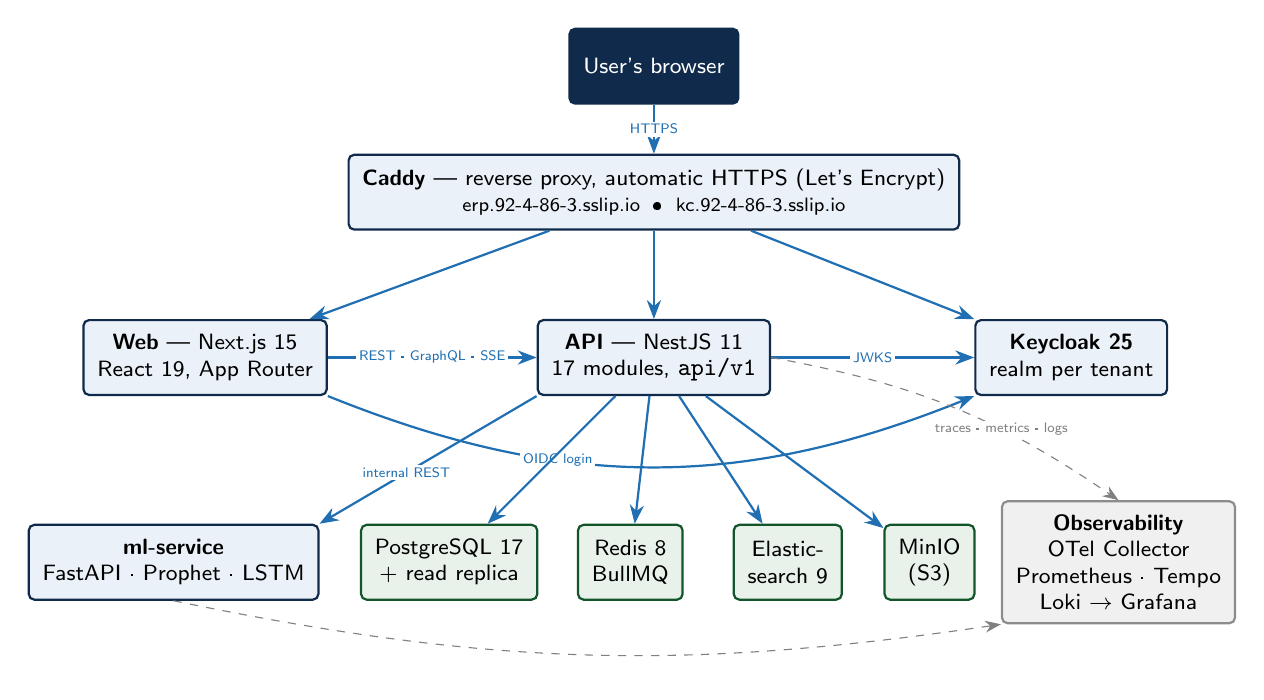
\begin{tikzpicture}[
  font=\sffamily\footnotesize,
  svc/.style={draw=amdoxnavy, thick, rounded corners=2pt, fill=amdoxlight, align=center, minimum height=0.95cm, inner sep=5pt},
  edge node/.style={font=\sffamily\tiny},
  data/.style={draw=okgreen!70!black, thick, rounded corners=2pt, fill=okgreen!10, align=center, minimum height=0.95cm, inner sep=5pt},
  obs/.style={draw=black!45, thick, rounded corners=2pt, fill=black!6, align=center, inner sep=5pt},
  arr/.style={-{Stealth[length=2.4mm]}, thick, color=amdoxblue},
  darr/.style={-{Stealth[length=2mm]}, thin, dashed, color=black!50},
  lab/.style={font=\sffamily\tiny, fill=white, inner sep=1pt},
]
  % client + proxy
  \node[svc, fill=amdoxnavy, text=white] (browser) at (0,0) {User's browser};
  \node[svc] (caddy) at (0,-1.6) {\textbf{Caddy} --- reverse proxy, automatic HTTPS (Let's Encrypt)\\
    \scriptsize erp.92-4-86-3.sslip.io \;\textbullet\; kc.92-4-86-3.sslip.io};
  % service row
  \node[svc] (web) at (-5.7,-3.7) {\textbf{Web} --- Next.js 15\\React 19, App Router};
  \node[svc] (api) at (0,-3.7) {\textbf{API} --- NestJS 11\\17 modules, \code{api/v1}};
  \node[svc] (kc)  at (5.3,-3.7) {\textbf{Keycloak 25}\\realm per tenant};
  % data + ML row
  \node[svc]  (ml)    at (-6.1,-6.3) {\textbf{ml-service}\\FastAPI · Prophet · LSTM};
  \node[data] (pg)    at (-2.6,-6.3) {PostgreSQL 17\\+ read replica};
  \node[data] (redis) at (-0.3,-6.3) {Redis 8\\BullMQ};
  \node[data] (es)    at (1.7,-6.3)  {Elastic-\\search 9};
  \node[data] (minio) at (3.5,-6.3)  {MinIO\\(S3)};
  % observability
  \node[obs] (otel) at (5.9,-6.3) {\textbf{Observability}\\OTel Collector\\Prometheus · Tempo\\Loki $\rightarrow$ Grafana};
  % arrows
  \draw[arr] (browser) -- node[lab]{HTTPS} (caddy);
  \draw[arr] (caddy) -- (web);
  \draw[arr] (caddy) -- (api);
  \draw[arr] (caddy) -- (kc);
  \draw[arr] (web) -- node[lab]{REST · GraphQL · SSE} (api);
  \draw[arr] (web.south east) to[bend right=22] node[lab, pos=0.35]{OIDC login} (kc.south west);
  \draw[arr] (api) -- node[lab]{JWKS} (kc);
  \draw[arr] (api) -- (pg);
  \draw[arr] (api) -- (redis);
  \draw[arr] (api) -- (es);
  \draw[arr] (api) -- (minio);
  \draw[arr] (api.south west) -- node[lab, pos=0.6]{internal REST} (ml.north east);
  \draw[darr] (api.east) to[bend left=12] node[lab, pos=0.65]{traces · metrics · logs} (otel.north);
  \draw[darr] (ml.south) to[bend right=10] (otel.south west);
\end{tikzpicture}
\caption{Deployed system topology. Everything runs on one Oracle Cloud VM: web/API/ml-service as
pm2-managed production builds, the data and identity layer as Docker containers, and the
observability stack as a separate Docker Compose project.}
\label{fig:topology}
\end{figure}

\subsection{Monorepo}

The repository is a Turborepo + pnpm workspace: \code{apps/web} (43 screens in Next.js
route groups), \code{apps/api}, \code{apps/ml-service}, and \code{packages/db} --- the
shared Prisma schema and the tenant-aware database client every module consumes.
\code{infra/} holds the operational estate: Docker Compose stacks (dev, prod,
observability), the Helm chart, ArgoCD manifests, and pm2 process configs.
Conventional commits are enforced by commitlint + Husky, and ESLint/Prettier run
repo-wide with zero violations.

\subsection{Multi-Tenant Design}

Tenancy is enforced at three independent layers, so a single mistake cannot leak data
across companies:

\begin{enumerate}
  \item \textbf{Identity} --- every tenant gets its \emph{own Keycloak realm}, created
  programmatically at signup, with realm roles (SuperAdmin, TenantAdmin, Manager, Viewer,
  Employee). Login discovers the home realm from the tenant slug; Google/SSO logins
  auto-link to existing accounts by verified e-mail, and a per-tenant \textbf{MFA toggle}
  forces OTP enrolment for every user in that tenant.
  \item \textbf{Request context} --- a \code{TenantContextInterceptor} extracts the tenant
  from the validated JWT and stores it in \code{AsyncLocalStorage}, making it available to
  any code on the request path without parameter threading.
  \item \textbf{Data} --- the shared Prisma client is wrapped with \code{\$extends()} logic
  that \emph{auto-injects} \code{tenantId} into every query's \code{where}/\code{data}.
  All 38 services use this client, and a custom TypeScript-AST static analyzer runs
  \textbf{in CI as a permanent gate}, failing the build if any query lacks tenant scoping
  (Section~\ref{sec:security} covers the two real cross-tenant bugs it caught).
\end{enumerate}

Beyond isolation, tenants are commercially separable: a \code{ModuleGuard} reads
per-tenant module licensing, so individual ERP modules can be switched on or off per
customer --- an extra the TDD did not require but which makes the platform genuinely
sellable as SaaS.

\subsection{Design Patterns in Use}

\begin{table}[H]
\centering\small
\renewcommand{\arraystretch}{1.3}
\begin{tabularx}{\textwidth}{l X}
\toprule
\rowcolor{amdoxnavy} \textcolor{white}{\textbf{Pattern}} & \textcolor{white}{\textbf{Where it earns its keep}} \\
Domain events & Modules never call each other directly: SCM emits \code{goods.received}; Finance's bridge listener reacts. Segregation of duties falls out of the design --- SCM cannot approve or pay invoices. \\
\rowcolor{amdoxlight}
Outbox & Finance writes \code{OutboxEvent} rows in the \emph{same transaction} as the business change; a BullMQ worker delivers them --- no lost events on a crash. \\
Saga w/ compensation & Payroll runs process 500-employee chunks asynchronously; a failed run \emph{wipes its partial payslips} before retrying (the fix proven by \code{verify:payroll-retry}). \\
\rowcolor{amdoxlight}
Guards \& decorators & \code{@Roles()} + RolesGuard on all business controllers (78 declarations); ModuleGuard for licensing; global validation pipe with class-validator DTOs. \\
Auto-posting listeners & GL subscribes to \code{invoice.approved}, \code{payment.made}, \code{payroll.completed}, \ldots{} and posts balanced journal entries idempotently (duplicate-checked on source module + ID). \\
\bottomrule
\end{tabularx}
\end{table}

\subsection{Data Model}

The schema comprises \textbf{67 Prisma models} on PostgreSQL~17, organised into ten
domains (Figure~\ref{fig:erd}). Conventions applied throughout: UUID keys,
\code{Decimal(18,4)} for all money, UTC timestamps, soft deletes, and composite indexes
added where an 80{,}000-row \code{EXPLAIN ANALYZE} audit proved they pay off.

\begin{figure}[p]
\centering
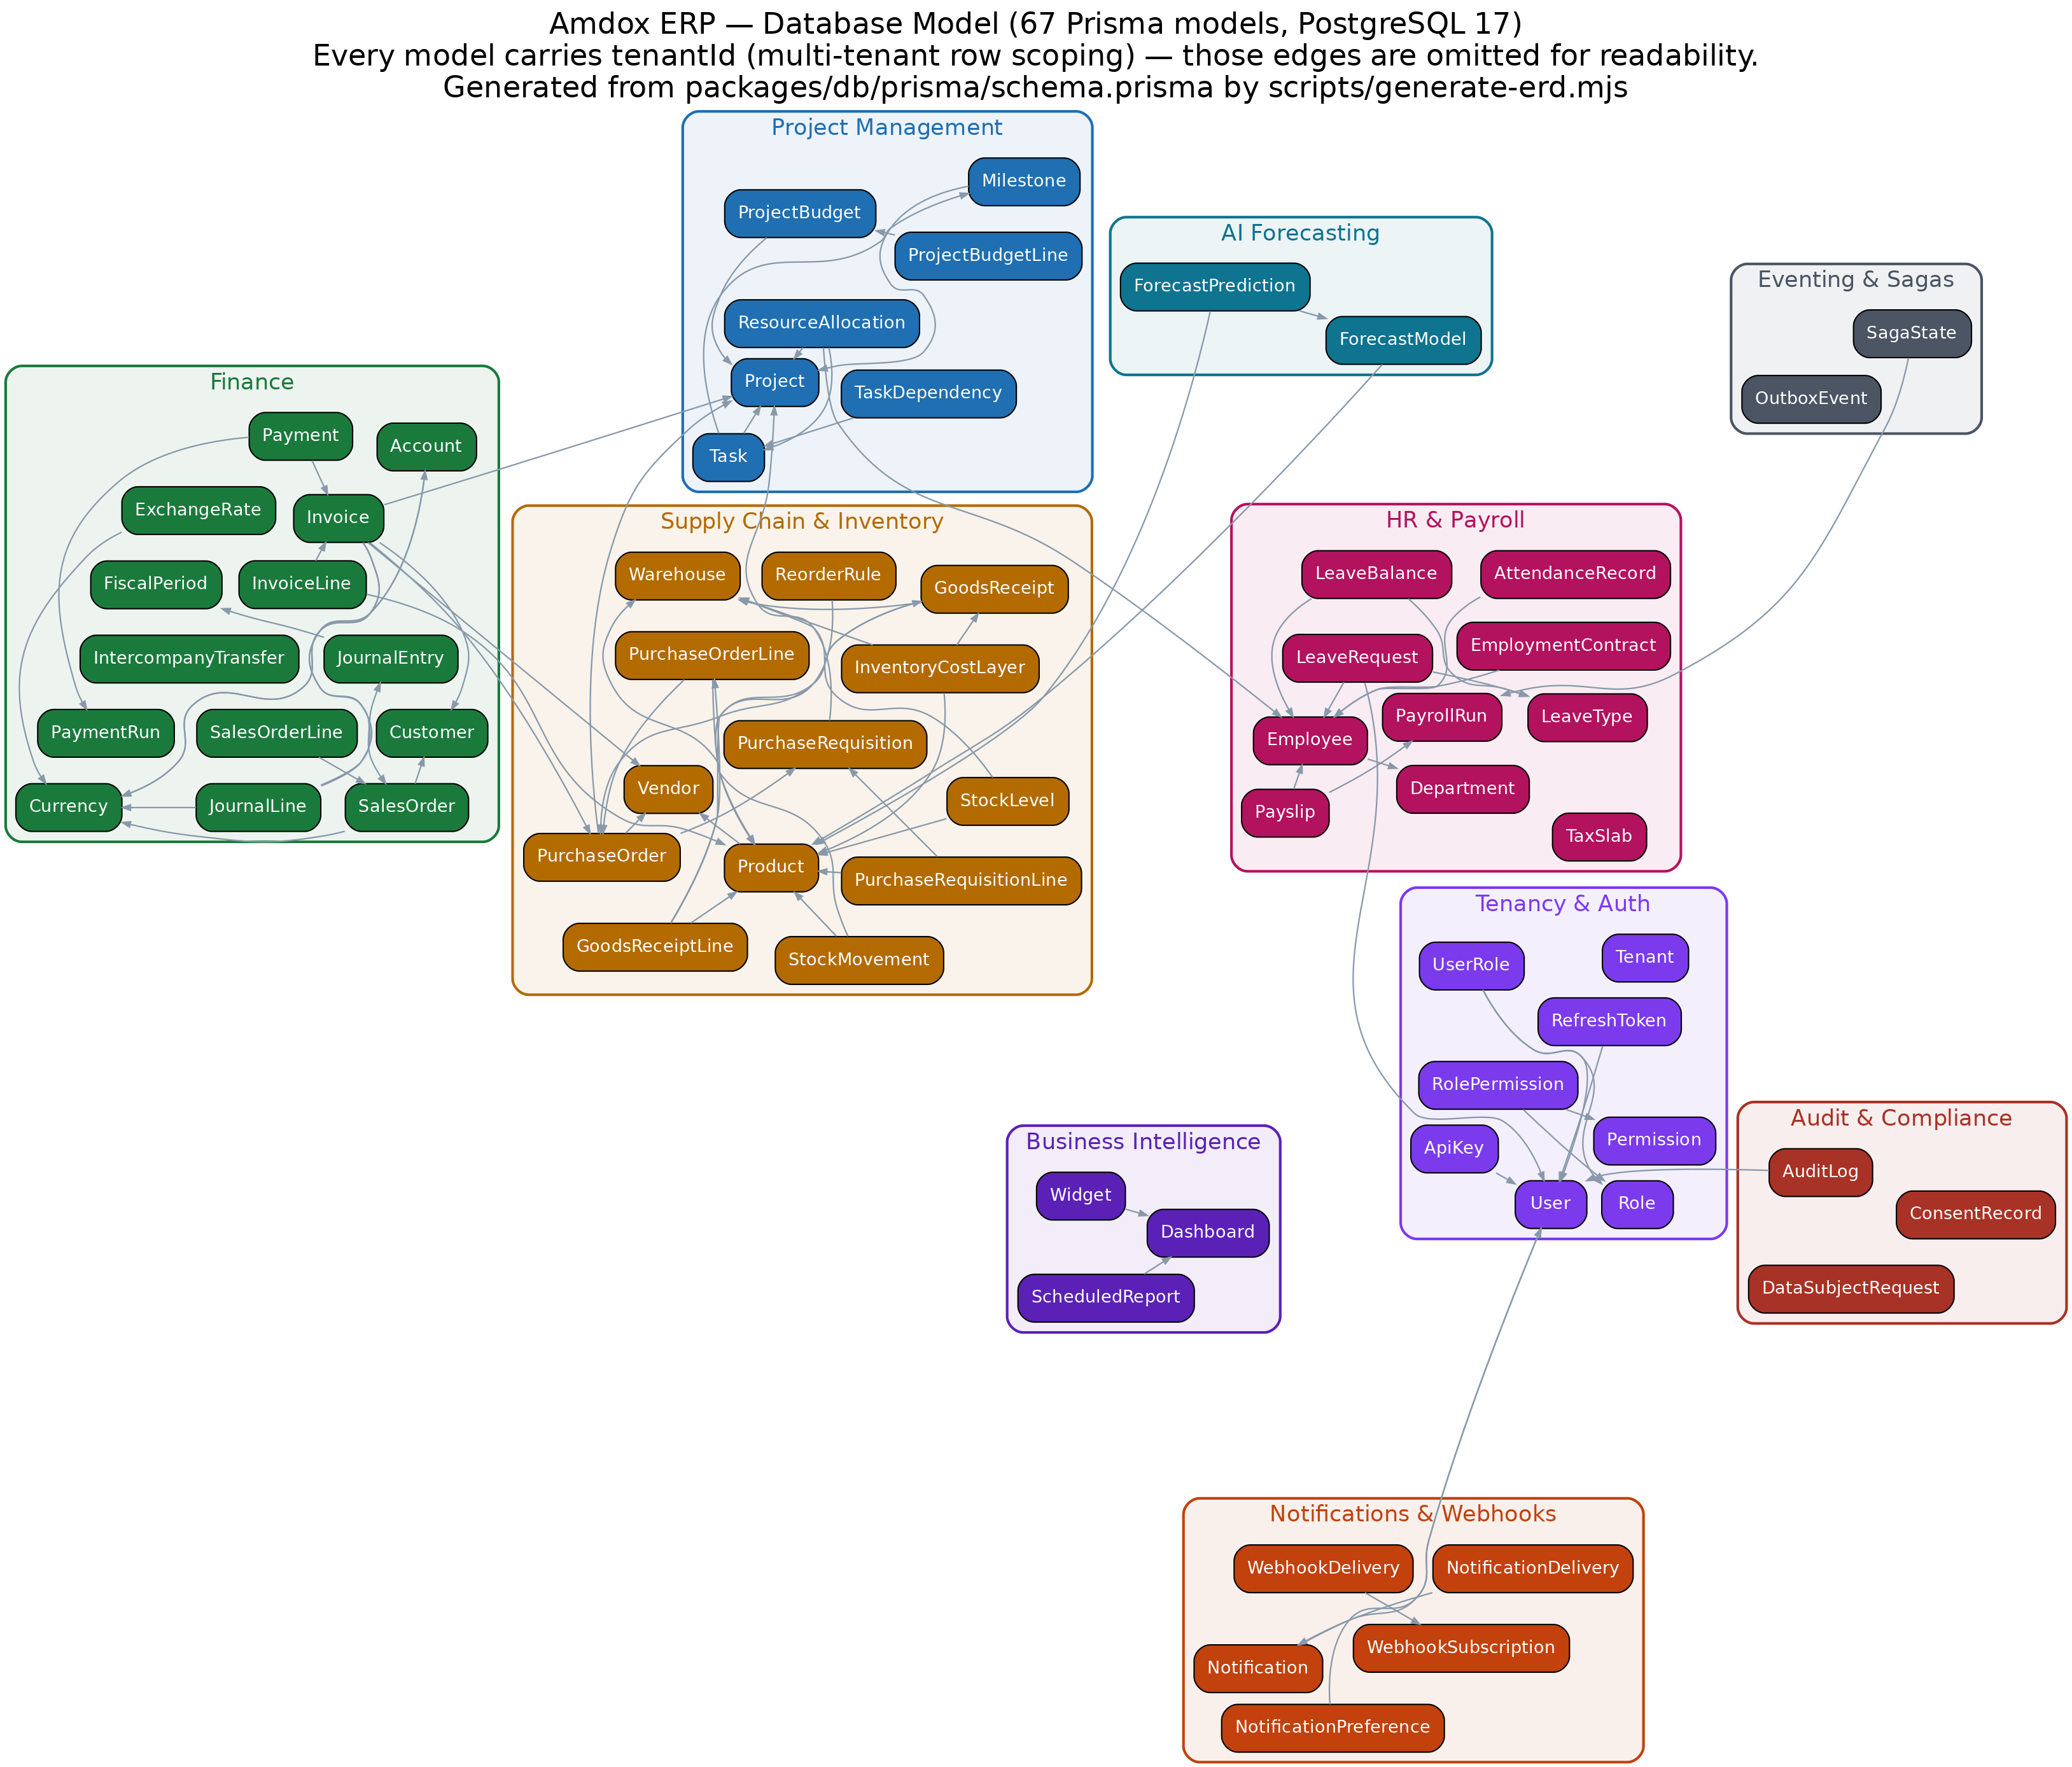
\includegraphics[width=\textwidth]{erd.png}
\caption{Database model --- 67 models, 77 relations, grouped by domain. Every model
carries \code{tenantId}; tenant-scoping edges are omitted for clarity.}
\label{fig:erd}
\end{figure}

% =====================================================================
\section{Functional Modules}\label{sec:modules}
% =====================================================================

\subsection{Authentication \& Identity (F-01)}

The auth module integrates \textbf{Keycloak 25} as the identity broker. Every new
tenant triggers a call to the Keycloak Admin API that creates a dedicated realm,
provisions the five system roles (SuperAdmin, TenantAdmin, Manager, Viewer, Employee),
and configures the OIDC client for the web app. Three login paths converge into a
single token:

\begin{itemize}
  \item \textbf{Path A --- Username/password:} standard Keycloak login form.
  \item \textbf{Path B --- Personal Google:} Google OAuth identity provider added per
  realm; on first login an account is created and auto-linked by verified email so the
  user never sees a conflict screen.
  \item \textbf{Path C --- Corporate SSO:} Keycloak's broker supports SAML and OIDC
  external IdPs (Azure AD, Google Workspace) --- plumbing is in place and tested with a
  Keycloak-to-Keycloak federation.
\end{itemize}

After login, every API call carries a short-lived RS256 JWT. The \code{KeycloakStrategy}
validates the signature against the realm's JWKS endpoint, maps the \code{ssoSubject} to
a local \code{User} record, and loads tenant + roles into \code{req.user}. A
\textbf{per-tenant MFA toggle} (Settings $\rightarrow$ Authentication) adds
\code{Configure~OTP} as a required action for every user in that realm, enforcing
TOTP on both password and SSO login paths. Token blacklisting on logout is implemented
via a Redis set that every guarded route checks.

\begin{figure}[H]
\centering
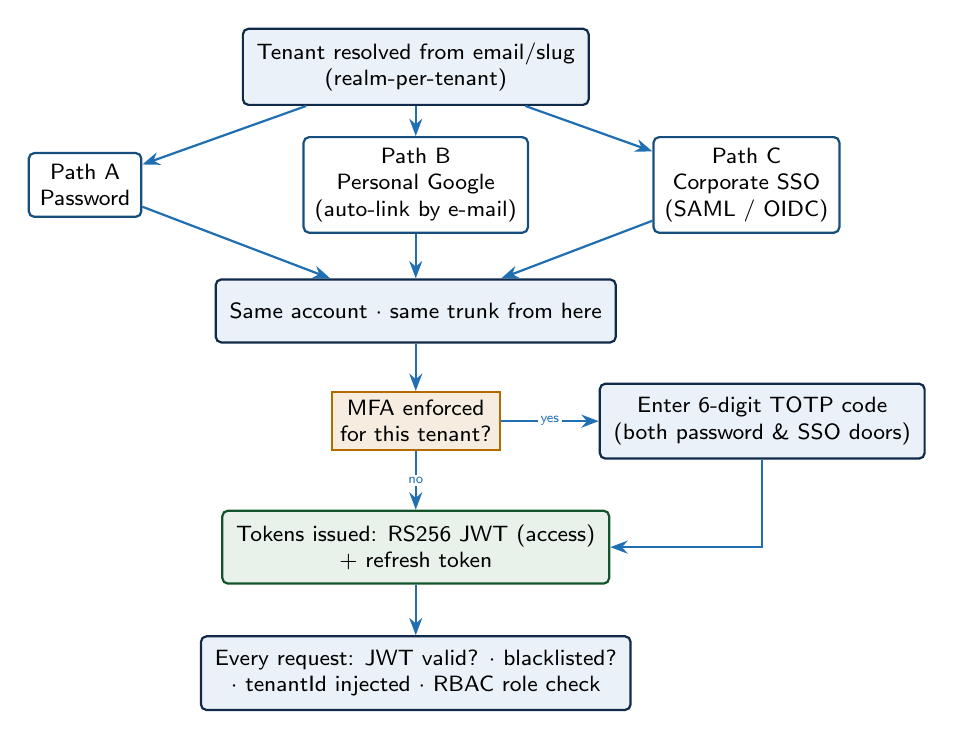
\begin{tikzpicture}[
  font=\sffamily\footnotesize,
  stp/.style={draw=amdoxnavy, thick, rounded corners=2pt, fill=amdoxlight, align=center, inner sep=5pt, minimum height=0.8cm},
  path/.style={draw=amdoxblue!70!black, thick, rounded corners=2pt, fill=white, align=center, inner sep=4pt, minimum height=0.8cm},
  dec/.style={draw=warnamber, thick, fill=warnamber!12, align=center, inner sep=3pt},
  done/.style={draw=okgreen!70!black, thick, rounded corners=2pt, fill=okgreen!10, align=center, inner sep=5pt, minimum height=0.8cm},
  arr/.style={-{Stealth[length=2.2mm]}, thick, color=amdoxblue},
  lab/.style={font=\sffamily\tiny, fill=white, inner sep=1pt},
]
  \node[stp] (tenant) at (0,0) {Tenant resolved from email/slug\\(realm-per-tenant)};
  \node[path] (a) at (-4.2,-1.5) {Path A\\Password};
  \node[path] (b) at (0,-1.5)    {Path B\\Personal Google\\(auto-link by e-mail)};
  \node[path] (c) at (4.2,-1.5)  {Path C\\Corporate SSO\\(SAML / OIDC)};
  \node[stp] (merge) at (0,-3.1) {Same account $\cdot$ same trunk from here};
  \node[dec]  (mfa) at (0,-4.5)   {MFA enforced\\for this tenant?};
  \node[stp] (otp) at (4.4,-4.5) {Enter 6-digit TOTP code\\(both password \& SSO doors)};
  \node[done] (tokens) at (0,-6.1) {Tokens issued: RS256 JWT (access)\\+ refresh token};
  \node[stp] (guard) at (0,-7.7) {Every request: JWT valid? $\cdot$ blacklisted?\\$\cdot$ tenantId injected $\cdot$ RBAC role check};
  \draw[arr] (tenant) -- (a); \draw[arr] (tenant) -- (b); \draw[arr] (tenant) -- (c);
  \draw[arr] (a) -- (merge); \draw[arr] (b) -- (merge); \draw[arr] (c) -- (merge);
  \draw[arr] (merge) -- (mfa);
  \draw[arr] (mfa) -- node[lab]{yes} (otp);
  \draw[arr] (mfa) -- node[lab]{no} (tokens);
  \draw[arr] (otp) |- (tokens);
  \draw[arr] (tokens) -- (guard);
\end{tikzpicture}
\caption{Authentication flow. Paths A/B/C are three ways to prove identity; everything
from the merge point on --- MFA, tokens, per-request guards --- is identical regardless
of path (adapted from \code{docs/architecture/auth-flow.md}).}
\end{figure}

\subsection{Financial Ledger --- GL (F-02)}

\begin{figure}[H]
\centering
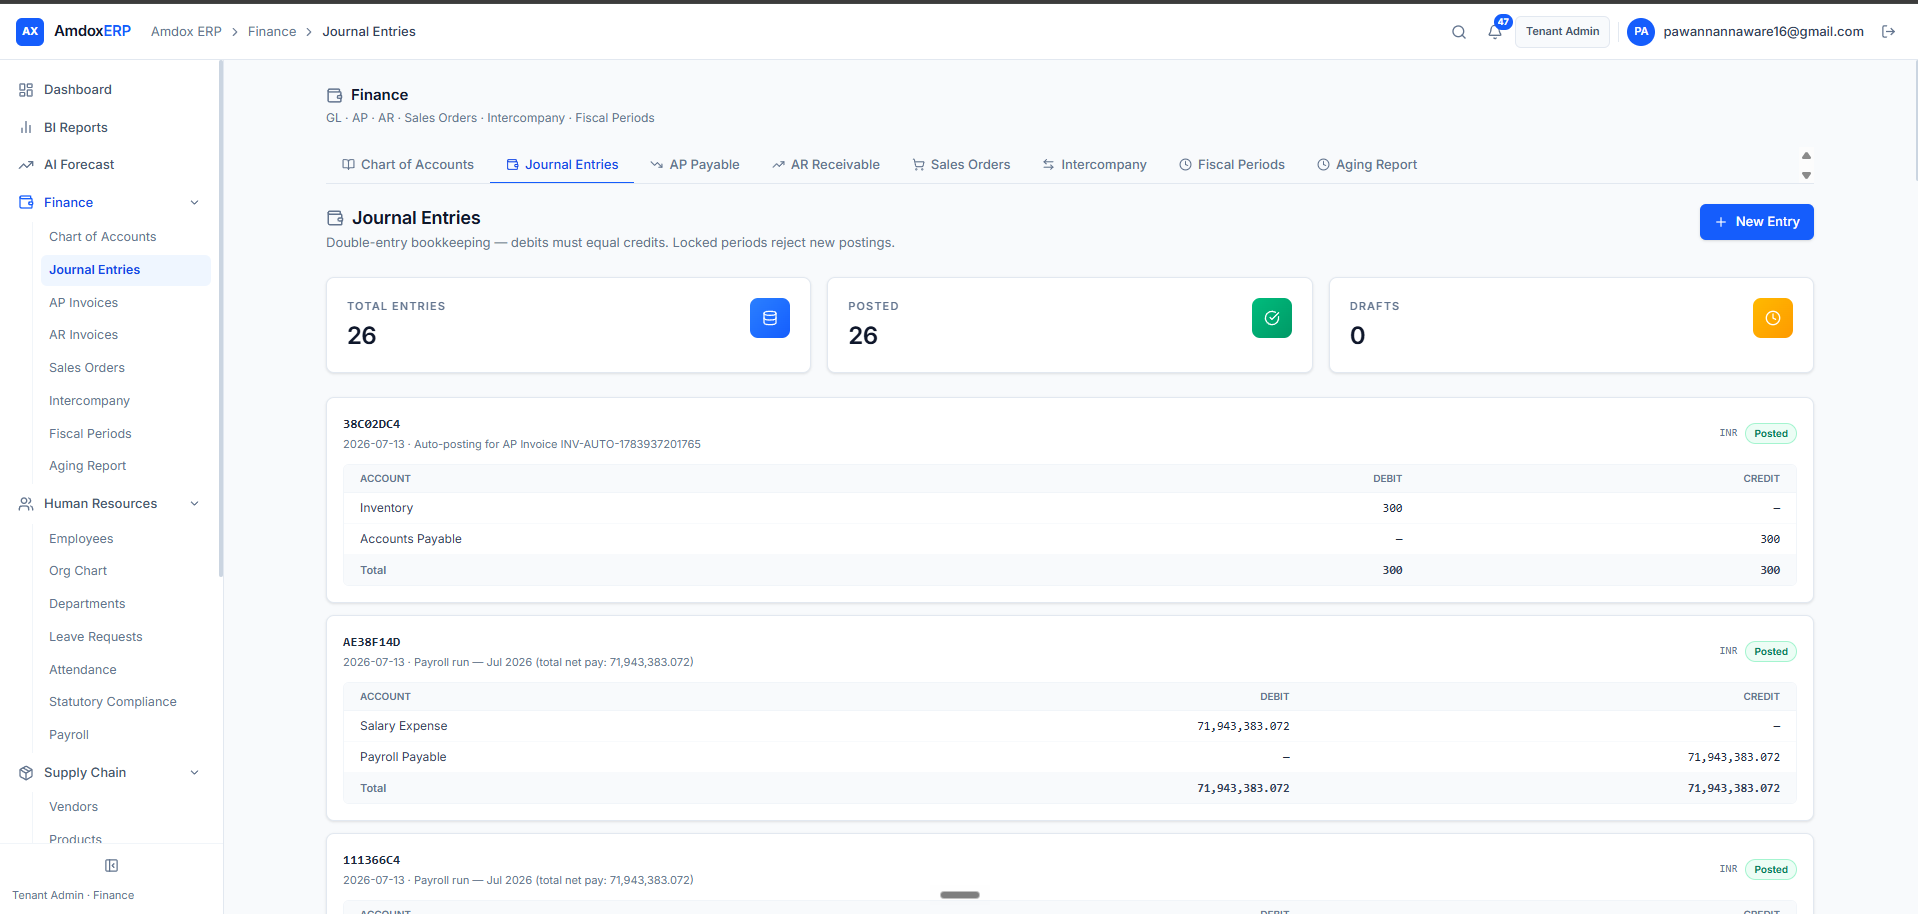
\includegraphics[width=0.92\textwidth]{journal-entry-form.png}
\caption{GL journal-entry creation screen. Debit/credit balancing is enforced by both
the UI and the \code{GlService} before persistence.}
\end{figure}

The General Ledger (\code{gl.service.ts}) enforces three accounting invariants at the
service layer:

\begin{enumerate}
  \item \textbf{Double-entry:} \code{createJournalEntry} rejects any entry where
  $\Sigma\text{Debits} \neq \Sigma\text{Credits}$ with a 400 error before touching the
  database.
  \item \textbf{Period-close guard:} posting into a locked \code{FiscalPeriod} throws;
  periods auto-open on the first business day of each month via cron.
  \item \textbf{Idempotency:} each auto-posting listener checks
  (\code{sourceModule}, \code{sourceId}) before inserting, so a retry never creates a
  duplicate journal entry.
\end{enumerate}

Auto-posting listeners handle every financial event:

\begin{table}[H]
\centering\small
\renewcommand{\arraystretch}{1.25}
\begin{tabularx}{\textwidth}{l l X}
\toprule
\rowcolor{amdoxnavy} \textcolor{white}{\textbf{Event}} & \textcolor{white}{\textbf{Debit}} & \textcolor{white}{\textbf{Credit}} \\
\code{invoice.approved} (AP)  & 1300 Inventory & 2000 Accounts Payable \\
\rowcolor{amdoxlight}
\code{invoice.issued} (AR)    & 1200 Accounts Receivable & 4000 Revenue \\
\code{payment.received}       & 1000 Cash & 1200 Accounts Receivable \\
\rowcolor{amdoxlight}
\code{payment.made}           & 2000 Accounts Payable & 1000 Cash \\
\code{payroll.completed}      & 6000 Salary Expense & 2100 Payroll Payable \\
\bottomrule
\end{tabularx}
\caption{Automatic journal entries posted by the GL service on domain events.}
\end{table}

Foreign-exchange rates are fetched daily from the ECB feed (29 currencies, per-tenant
\code{ExchangeRate} rows); actual conversion in postings is on the roadmap.

\subsection{AP / AR Automation (F-03)}

\begin{figure}[H]
\centering
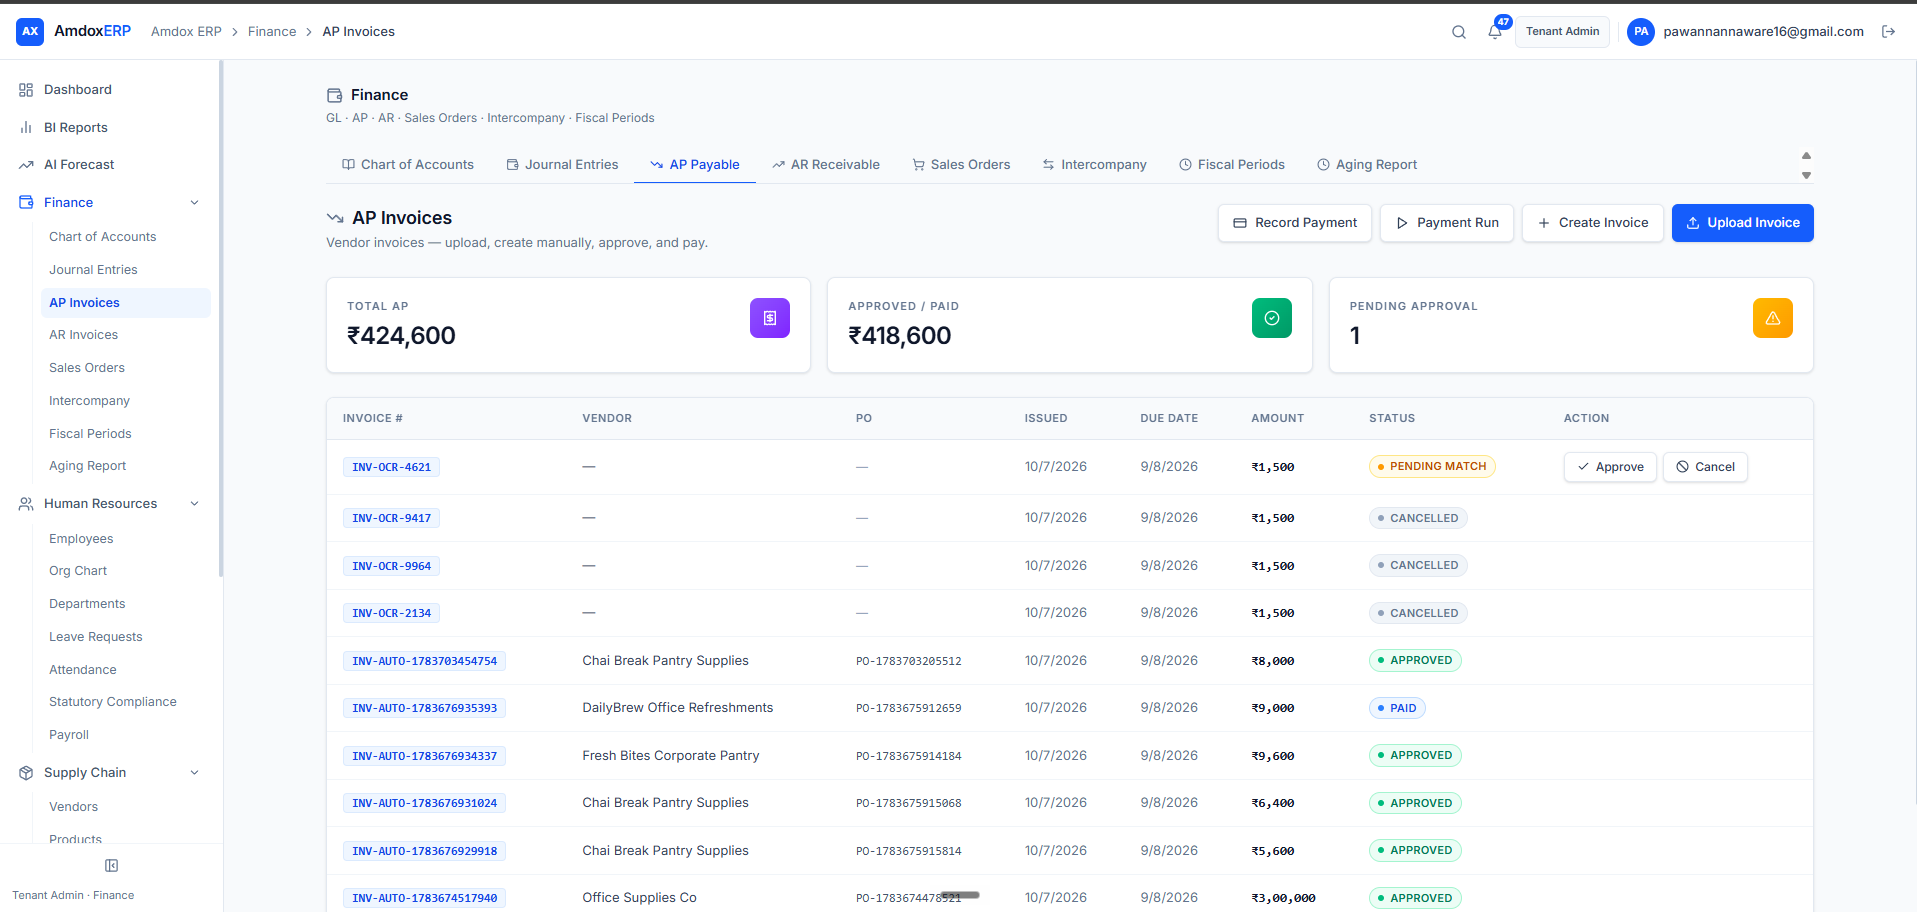
\includegraphics[width=0.92\textwidth]{ap-invoices.png}
\caption{Accounts Payable invoice list. Statuses (PENDING\_MATCH, APPROVED, PAID)
reflect 3-way match outcomes; the upload button triggers AWS Textract OCR.}
\end{figure}

\subsubsection*{Accounts Payable}
Invoice processing supports two entry paths:
\begin{itemize}
  \item \textbf{Auto-creation:} when a goods receipt is committed, the SCM--Finance
  bridge creates an AP invoice for the received quantities and immediately runs the
  3-way match.
  \item \textbf{Manual upload:} finance staff uploads a PDF; AWS Textract
  \code{AnalyzeExpense} extracts vendor, date, line items, and totals with per-field
  confidence scores (a local mock is the fallback when no AWS credentials are
  configured).
\end{itemize}

The \textbf{three-way match} (\code{performThreeWayMatch}) verifies:
(i)~invoice vendor matches PO vendor;
(ii)~per-line invoiced quantity $\leq$ received quantity;
(iii)~per-line unit price within $\pm$2\% of the PO line price
(header-total fallback when lines cannot be resolved to products).
A passing match auto-approves the invoice in under one second; a failure parks it as
\code{PENDING\_MATCH} for manual review. Payment runs batch-settle approved invoices
with per-invoice failure isolation and \code{PARTIALLY\_PAID} states.

\begin{figure}[H]
\centering
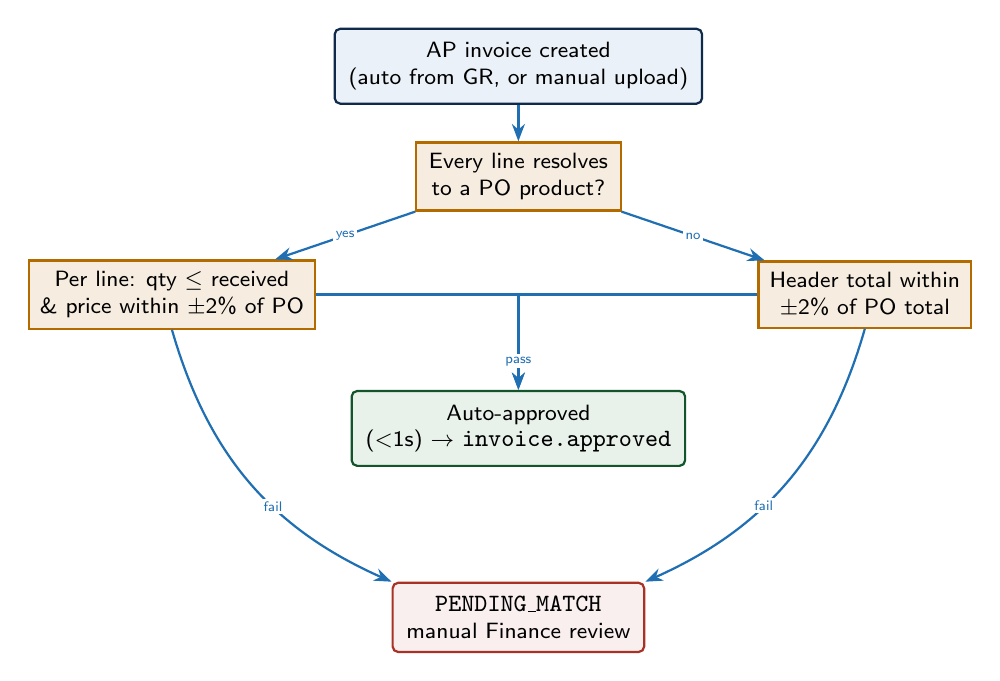
\begin{tikzpicture}[
  font=\sffamily\footnotesize,
  stp/.style={draw=amdoxnavy, thick, rounded corners=2pt, fill=amdoxlight, align=center, inner sep=5pt, minimum height=0.8cm},
  dec/.style={draw=warnamber, thick, fill=warnamber!12, align=center, inner sep=4pt, minimum width=2.6cm},
  pass/.style={draw=okgreen!70!black, thick, rounded corners=2pt, fill=okgreen!10, align=center, inner sep=5pt},
  fail/.style={draw=gapred, thick, rounded corners=2pt, fill=gapred!8, align=center, inner sep=5pt},
  arr/.style={-{Stealth[length=2.2mm]}, thick, color=amdoxblue},
  lab/.style={font=\sffamily\tiny, fill=white, inner sep=1pt},
]
  \node[stp] (start) at (0,0) {AP invoice created\\(auto from GR, or manual upload)};
  \node[dec]  (lines) at (0,-1.4) {Every line resolves\\to a PO product?};
  \node[dec]  (linecheck) at (-4.4,-2.9) {Per line: qty $\leq$ received\\\& price within $\pm$2\% of PO};
  \node[dec]  (headercheck) at (4.4,-2.9) {Header total within\\$\pm$2\% of PO total};
  \node[pass] (approve) at (0,-4.6) {Auto-approved\\($<$1s) $\rightarrow$ \code{invoice.approved}};
  \node[fail] (pending) at (0,-7.0) {\code{PENDING\_MATCH}\\manual Finance review};
  \draw[arr] (start) -- (lines);
  \draw[arr] (lines) -- node[lab]{yes} (linecheck);
  \draw[arr] (lines) -- node[lab]{no} (headercheck);
  \draw[arr] (linecheck) -| node[lab, pos=0.85]{pass} (approve);
  \draw[arr] (headercheck) -| node[lab, pos=0.85]{pass} (approve);
  \draw[arr] (linecheck.south) to[bend right=25] node[lab, pos=0.6]{fail} (pending.north west);
  \draw[arr] (headercheck.south) to[bend left=25] node[lab, pos=0.6]{fail} (pending.north east);
\end{tikzpicture}
\caption{Three-way match decision flow (\code{performThreeWayMatch}). Line-level
checking is preferred; header-total is a fallback when invoice lines cannot be mapped
to PO products.}
\end{figure}

\subsubsection*{Accounts Receivable}
Customers, AR invoices, payment recording, and an \textbf{aging report} (grouping
outstanding balances by 0--30, 31--60, 61--90, and $>$90 days) are all implemented.
A sales-order module provides the order-to-cash entry point: sales order $\rightarrow$
AR invoice $\rightarrow$ GL posts revenue.

\subsection{HR \& Payroll (F-04)}

\begin{figure}[H]
\centering
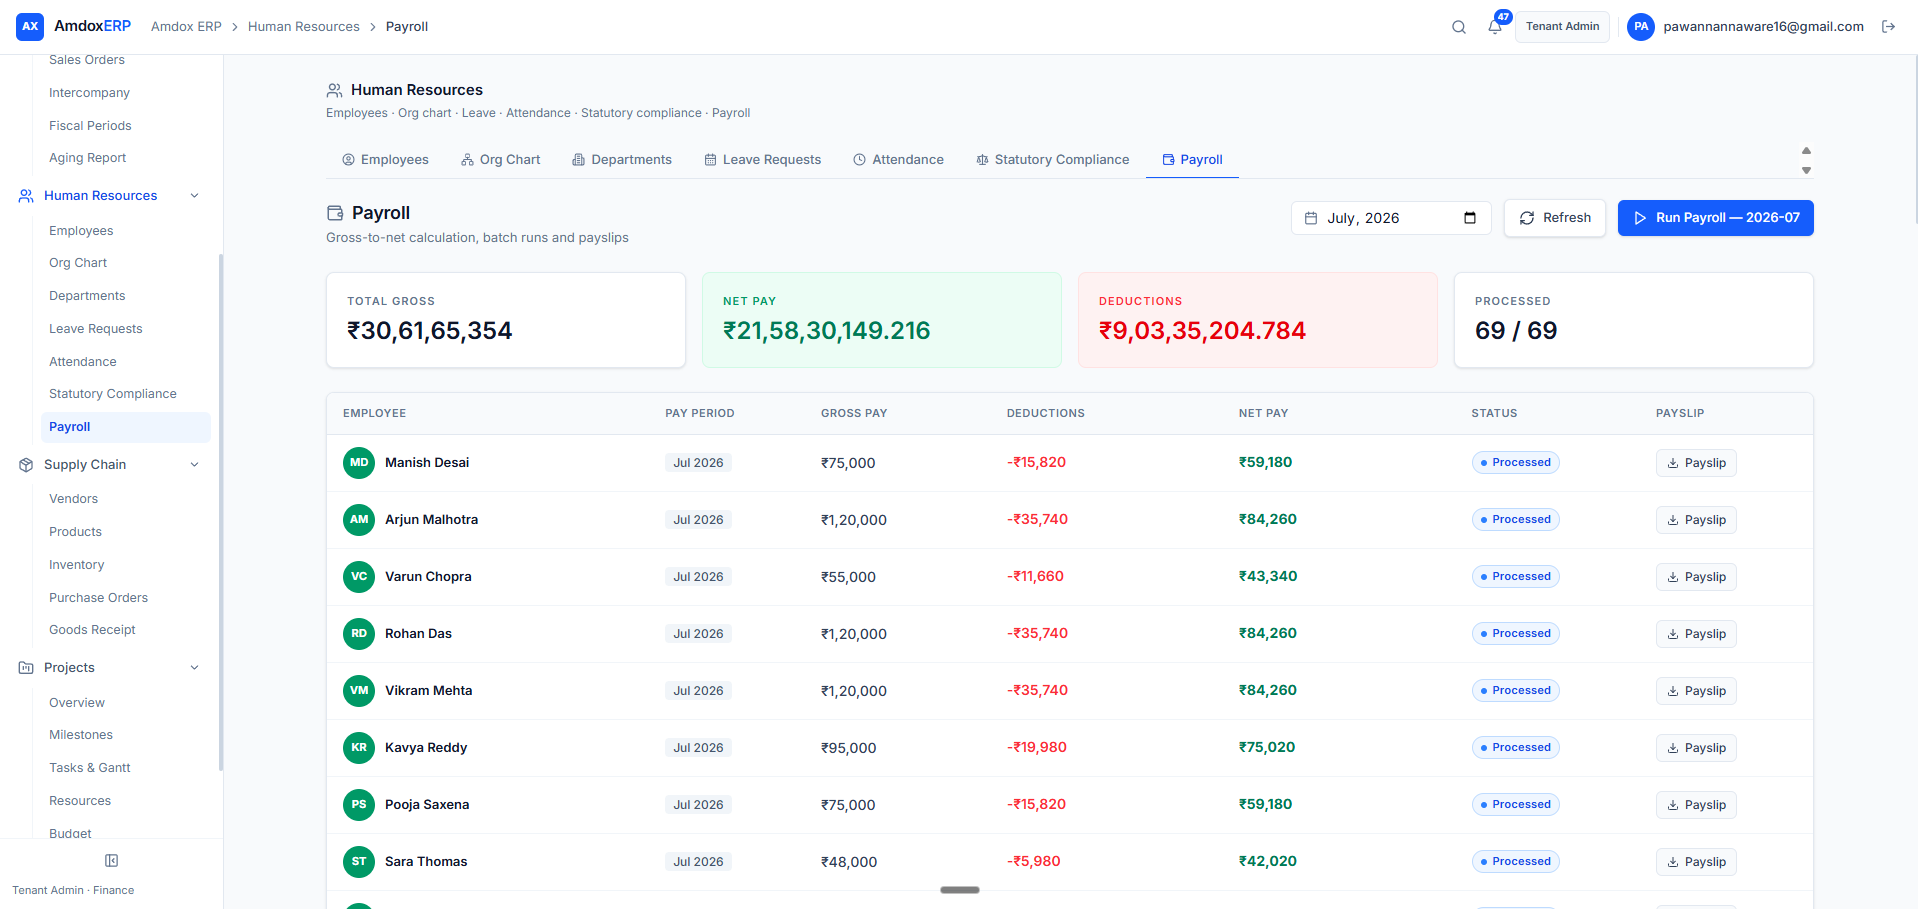
\includegraphics[width=0.92\textwidth]{payroll-run.png}
\caption{Payroll run dashboard. Each row shows gross pay, statutory deductions, and
net pay; the PDF payslip is downloadable from the same screen.}
\end{figure}

\subsubsection*{Employee Management}
Full CRUD with employment contracts (salary history), department hierarchy,
\code{managerId} tree, and soft-delete. Employees self-serve via \code{GET /hr/employees/me}
and a personal home-page dashboard (tabbed: Profile / Attendance \& Leave / Pay).

\subsubsection*{Leave Management}
A leave state-machine enforces: only the \emph{direct manager, an HR-department
approver, or a TenantAdmin} can approve or reject a leave request. The state-machine
is pure-function, making approval rules easy to unit-test in isolation.

\begin{figure}[H]
\centering
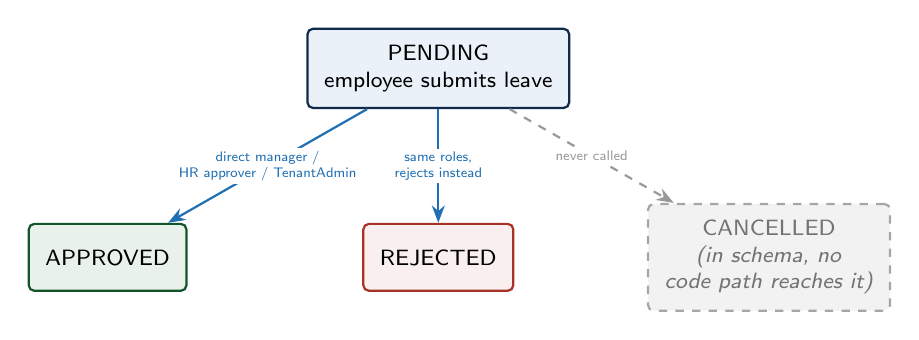
\begin{tikzpicture}[
  font=\sffamily\footnotesize,
  st/.style={draw=amdoxnavy, thick, rounded corners=2pt, fill=amdoxlight, align=center, inner sep=6pt, minimum height=0.85cm},
  term/.style={draw=okgreen!70!black, thick, rounded corners=2pt, fill=okgreen!10, align=center, inner sep=6pt, minimum height=0.85cm},
  rej/.style={draw=gapred, thick, rounded corners=2pt, fill=gapred!8, align=center, inner sep=6pt, minimum height=0.85cm},
  dead/.style={draw=black!35, thick, dashed, rounded corners=2pt, fill=black!5, align=center, inner sep=6pt, minimum height=0.85cm, text=black!55},
  arr/.style={-{Stealth[length=2.2mm]}, thick, color=amdoxblue},
  lab/.style={font=\sffamily\tiny, fill=white, inner sep=1pt},
]
  \node[st]   (pending) at (0,0)     {PENDING\\employee submits leave};
  \node[term] (approved) at (-4.2,-2.4) {APPROVED};
  \node[rej]  (rejected) at (0,-2.4)    {REJECTED};
  \node[dead] (cancelled) at (4.2,-2.4) {CANCELLED\\\emph{(in schema, no}\\\emph{code path reaches it)}};
  \draw[arr] (pending) -- node[lab, align=center]{direct manager /\\HR approver / TenantAdmin} (approved);
  \draw[arr] (pending) -- node[lab, align=center]{same roles,\\rejects instead} (rejected);
  \draw[arr, dashed, color=black!40] (pending) -- node[lab]{never called} (cancelled);
\end{tikzpicture}
\caption{Leave request state machine (\code{LeaveStateMachine.validateTransition}).
Only \code{PENDING} is a valid starting state; \code{APPROVED} and \code{REJECTED} are
terminal. Every transition re-checks authorization --- the caller must be the
employee's direct manager, an HR-department approver, or a TenantAdmin, or the service
throws \code{ForbiddenException}. \code{CANCELLED} is defined in the schema but has no
reachable code path --- a documented dead state, not a missing feature.}
\end{figure}

\subsubsection*{Attendance}
Clock-in/out records accumulate per-day overtime minutes; the payroll engine converts
these into overtime pay at 1.5$\times$ the hourly rate.

\subsubsection*{Payroll Engine}
A BullMQ worker processes runs asynchronously in \textbf{chunks of 500 employees}
for memory safety. The gross-to-net computation applies:
PF (12\% employee + 12\% employer on basic), ESI (0.75\% employee + 3.25\% employer,
under the \textrm{Rs.}~21{,}000 ceiling), Professional Tax, Labour Welfare Fund,
gratuity accrual, and TDS from per-tenant configurable tax slabs.
Generated payslip PDFs are stored in MinIO (S3-compatible). On completion, the
\code{payroll.completed} event posts the salary GL entry and credits each linked
project's labour-cost budget.

\begin{figure}[H]
\centering
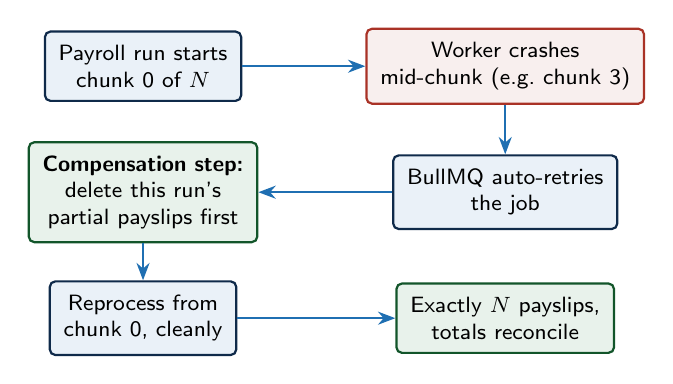
\begin{tikzpicture}[
  font=\sffamily\footnotesize,
  stp/.style={draw=amdoxnavy, thick, rounded corners=2pt, fill=amdoxlight, align=center, inner sep=5pt, minimum height=0.8cm},
  bad/.style={draw=gapred, thick, rounded corners=2pt, fill=gapred!8, align=center, inner sep=5pt},
  fix/.style={draw=okgreen!70!black, thick, rounded corners=2pt, fill=okgreen!10, align=center, inner sep=5pt},
  arr/.style={-{Stealth[length=2.2mm]}, thick, color=amdoxblue},
  lab/.style={font=\sffamily\tiny, fill=white, inner sep=1pt},
]
  \node[stp] (run) at (0,0)     {Payroll run starts\\chunk 0 of $N$};
  \node[bad]  (crash) at (4.6,0) {Worker crashes\\mid-chunk (e.g.\ chunk 3)};
  \node[stp] (retry) at (4.6,-1.6) {BullMQ auto-retries\\the job};
  \node[fix]  (comp) at (0,-1.6) {\textbf{Compensation step:}\\delete this run's\\partial payslips first};
  \node[stp] (restart) at (0,-3.2) {Reprocess from\\chunk 0, cleanly};
  \node[fix]  (done) at (4.6,-3.2) {Exactly $N$ payslips,\\totals reconcile};
  \draw[arr] (run) -- (crash);
  \draw[arr] (crash) -- (retry);
  \draw[arr] (retry) -- (comp);
  \draw[arr] (comp) -- (restart);
  \draw[arr] (restart) -- (done);
\end{tikzpicture}
\caption{Payroll saga compensation. Before the fix, a mid-run crash left chunk 0--2's
payslips in place and the retry re-inserted them --- 21 employees produced 42 payslips.
The compensation step (delete-before-reprocess) makes the retry idempotent, verified
live with \code{pnpm --filter api verify:payroll-retry}.}
\end{figure}

\subsection{Supply Chain Management (F-05)}

\begin{figure}[H]
\centering
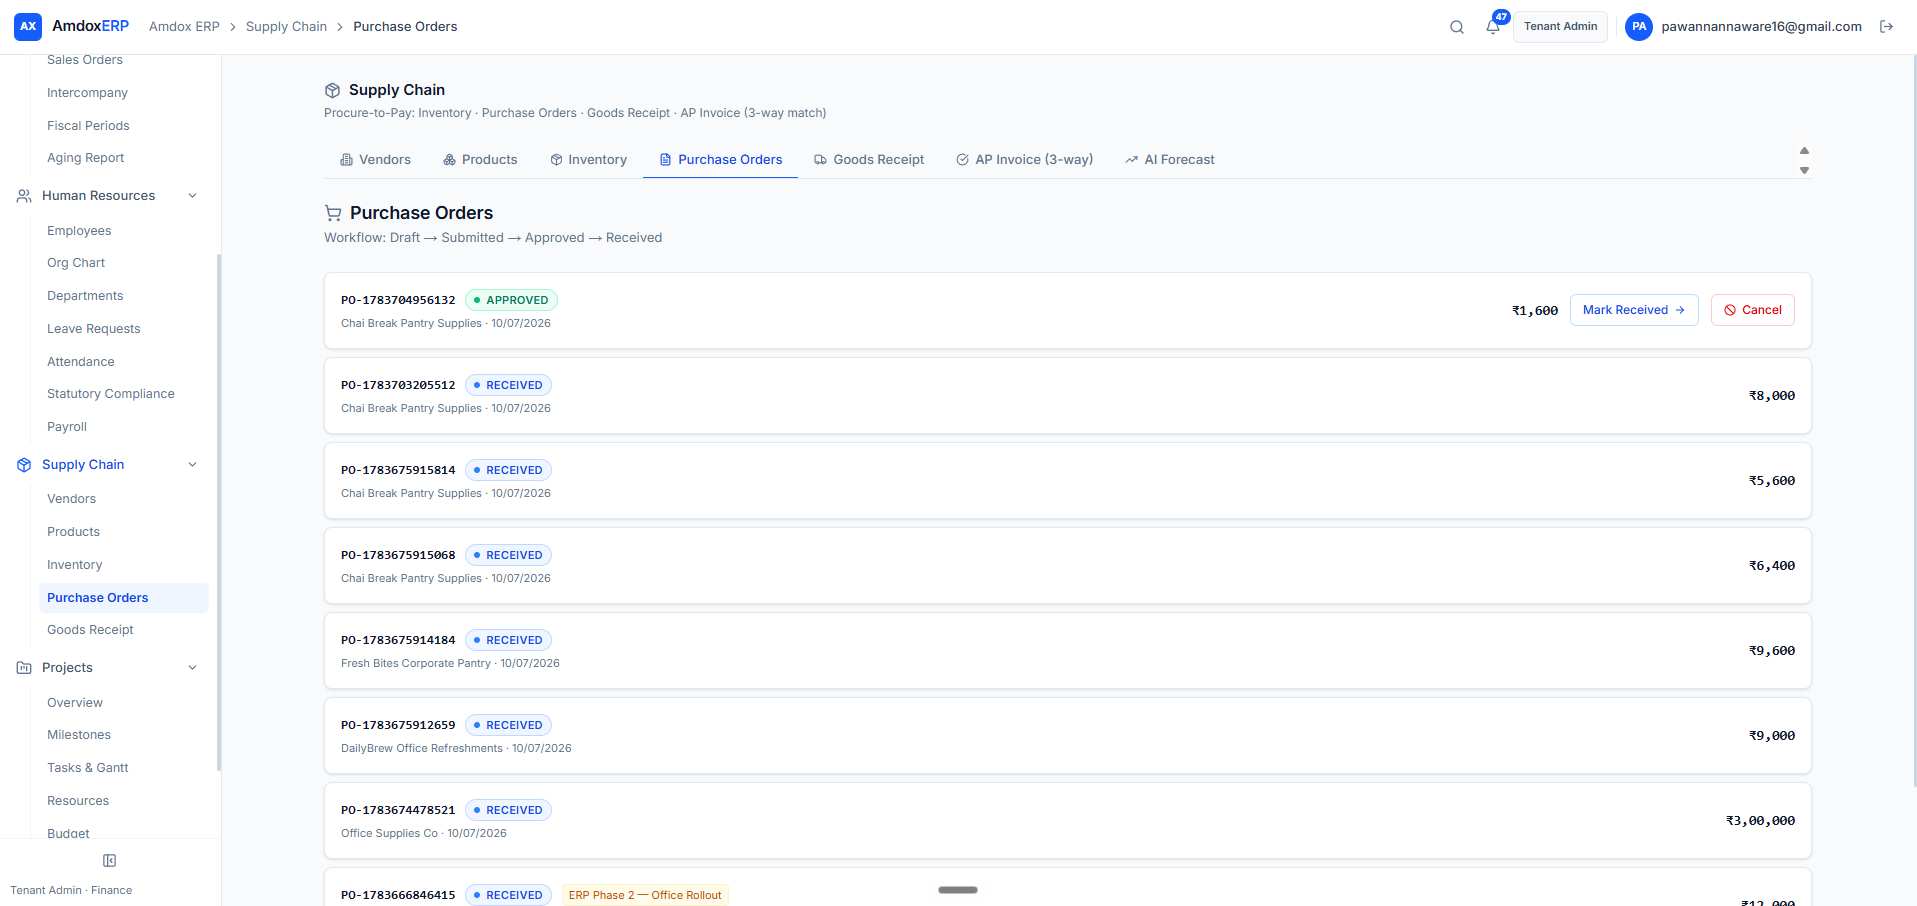
\includegraphics[width=0.92\textwidth]{purchase-orders.png}
\caption{Purchase Order list with status badges (DRAFT, APPROVED, RECEIVED). The
Goods Receipt button opens the per-line quantity capture dialog.}
\end{figure}

The SCM module spans the full procure-to-pay cycle:

\begin{itemize}
  \item \textbf{Vendors \& Products:} full CRUD; a vendor portal (pre-shared portal-key
  header auth, scoped to that vendor's own data) lets suppliers view their POs and post
  acknowledgements without an internal user account.
  \item \textbf{Requisition $\rightarrow$ PO:} purchase requisitions (from project
  managers or the reorder engine) are reviewed by supply-chain managers, who convert
  them to POs against a chosen vendor.
  \item \textbf{Goods Receipt:} supports full and \emph{partial} delivery --- each
  receipt records per-line quantities (\code{GoodsReceiptLine}), enabling the PO to
  remain \code{PARTIALLY\_RECEIVED} across multiple deliveries.
  \item \textbf{FIFO Inventory:} each goods receipt creates a cost layer; outbound stock
  movements consume oldest layers first, giving accurate weighted-average cost of goods
  sold.
  \item \textbf{Reorder Automation:} configurable reorder points per product/warehouse;
  the scheduler auto-drafts a purchase requisition whenever stock falls below the
  threshold.
\end{itemize}

\subsection{AI Demand Forecasting (F-06)}

The \textbf{ml-service} (Python FastAPI) runs two models per SKU:
\textbf{Prophet} for products with seasonal/trend patterns, and a \textbf{PyTorch LSTM}
for high-volume SKUs. Predictions are cached in Redis and served to the API via
internal REST. A weekly \code{forecast-retrain} BullMQ job pulls fresh sales and stock
data, retrains models, and invalidates the cache. If MAPE exceeds 12\%, the service
emits a \code{forecast.mape\_breach} event that triggers an alert to supply-chain
managers.

\begin{figure}[H]
\centering
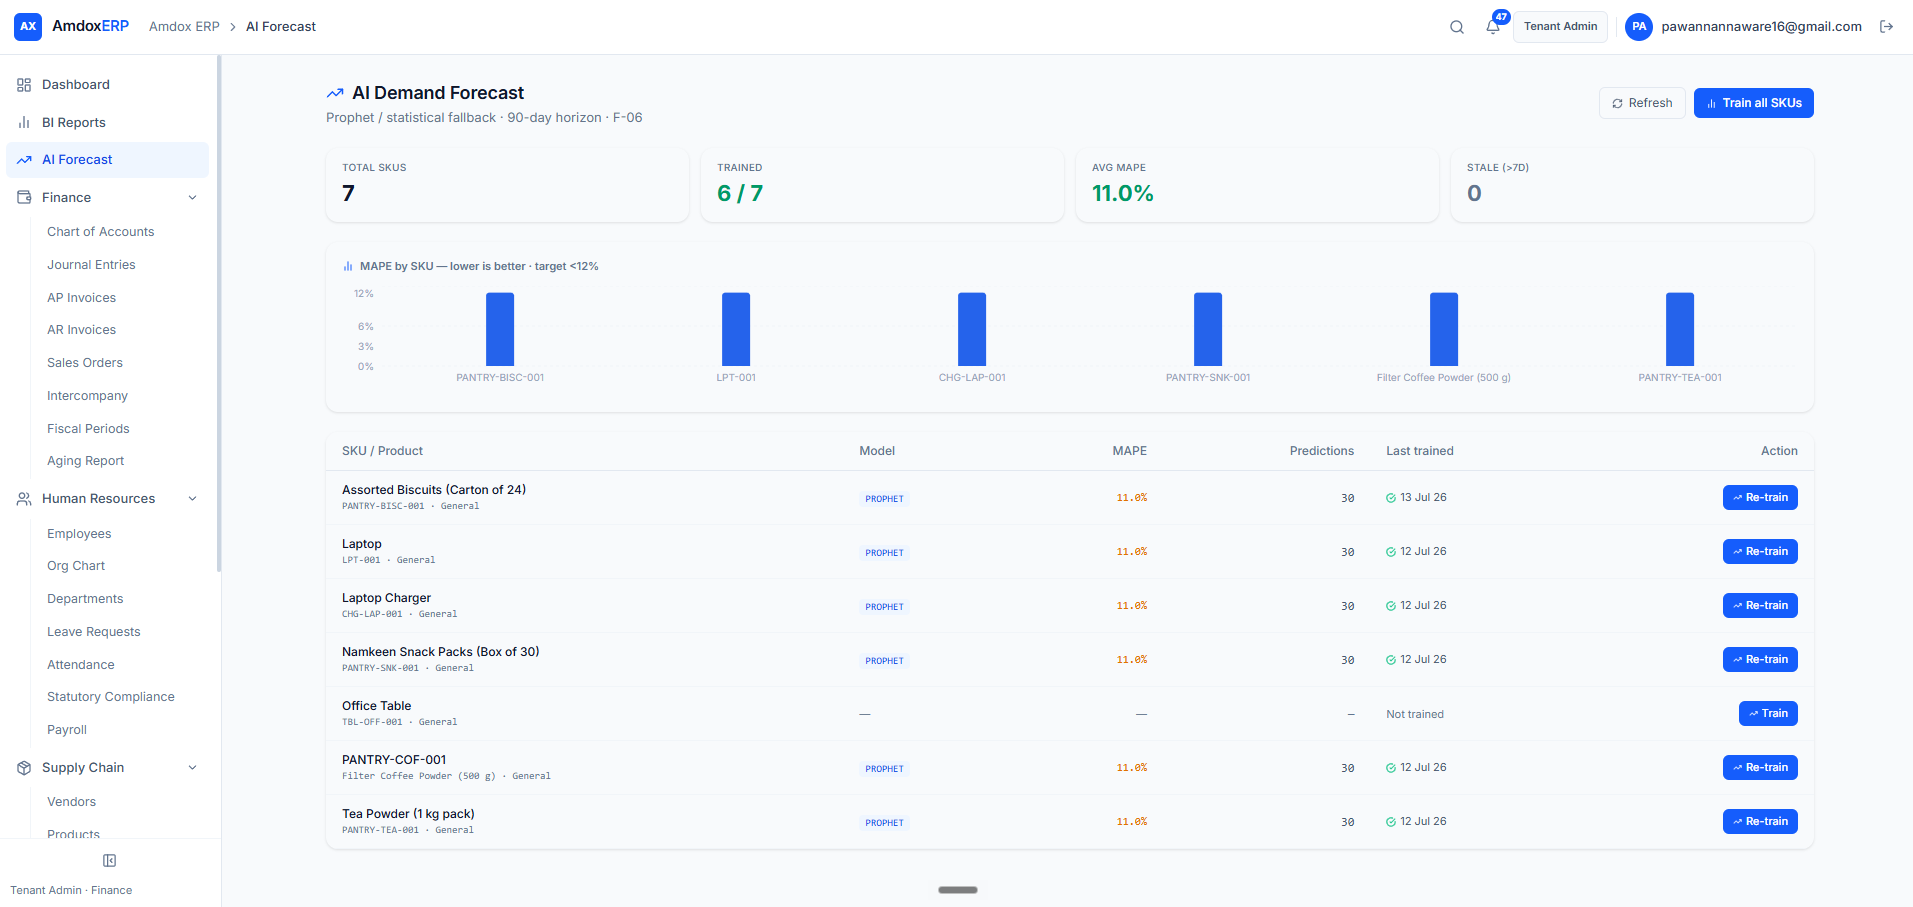
\includegraphics[width=0.92\textwidth]{forecast.png}
\caption{Demand forecast chart for a sample SKU --- 90-day prediction with
confidence bands (80\% and 95\%), actual vs.\ predicted overlay, and model MAPE display.}
\end{figure}

\subsection{Project Management (F-07)}

Projects move through a lifecycle (Planning $\rightarrow$ Active $\rightarrow$
On Hold $\rightarrow$ Closed). Key capabilities include:
DAG-validated task dependencies (cycle detection on save), an interactive
\textbf{Gantt chart}, a resource-utilisation heatmap, and milestone tracking.
Budget actuals are fed automatically from two sources: approved AP invoices whose PO
carries a \code{projectId}, and payroll runs that credit labour costs from resource
allocations. When actuals exceed budget by $>$10\%, an overrun alert fires through
the notification engine.

\subsection{Business Intelligence (F-08)}

\begin{figure}[H]
\centering
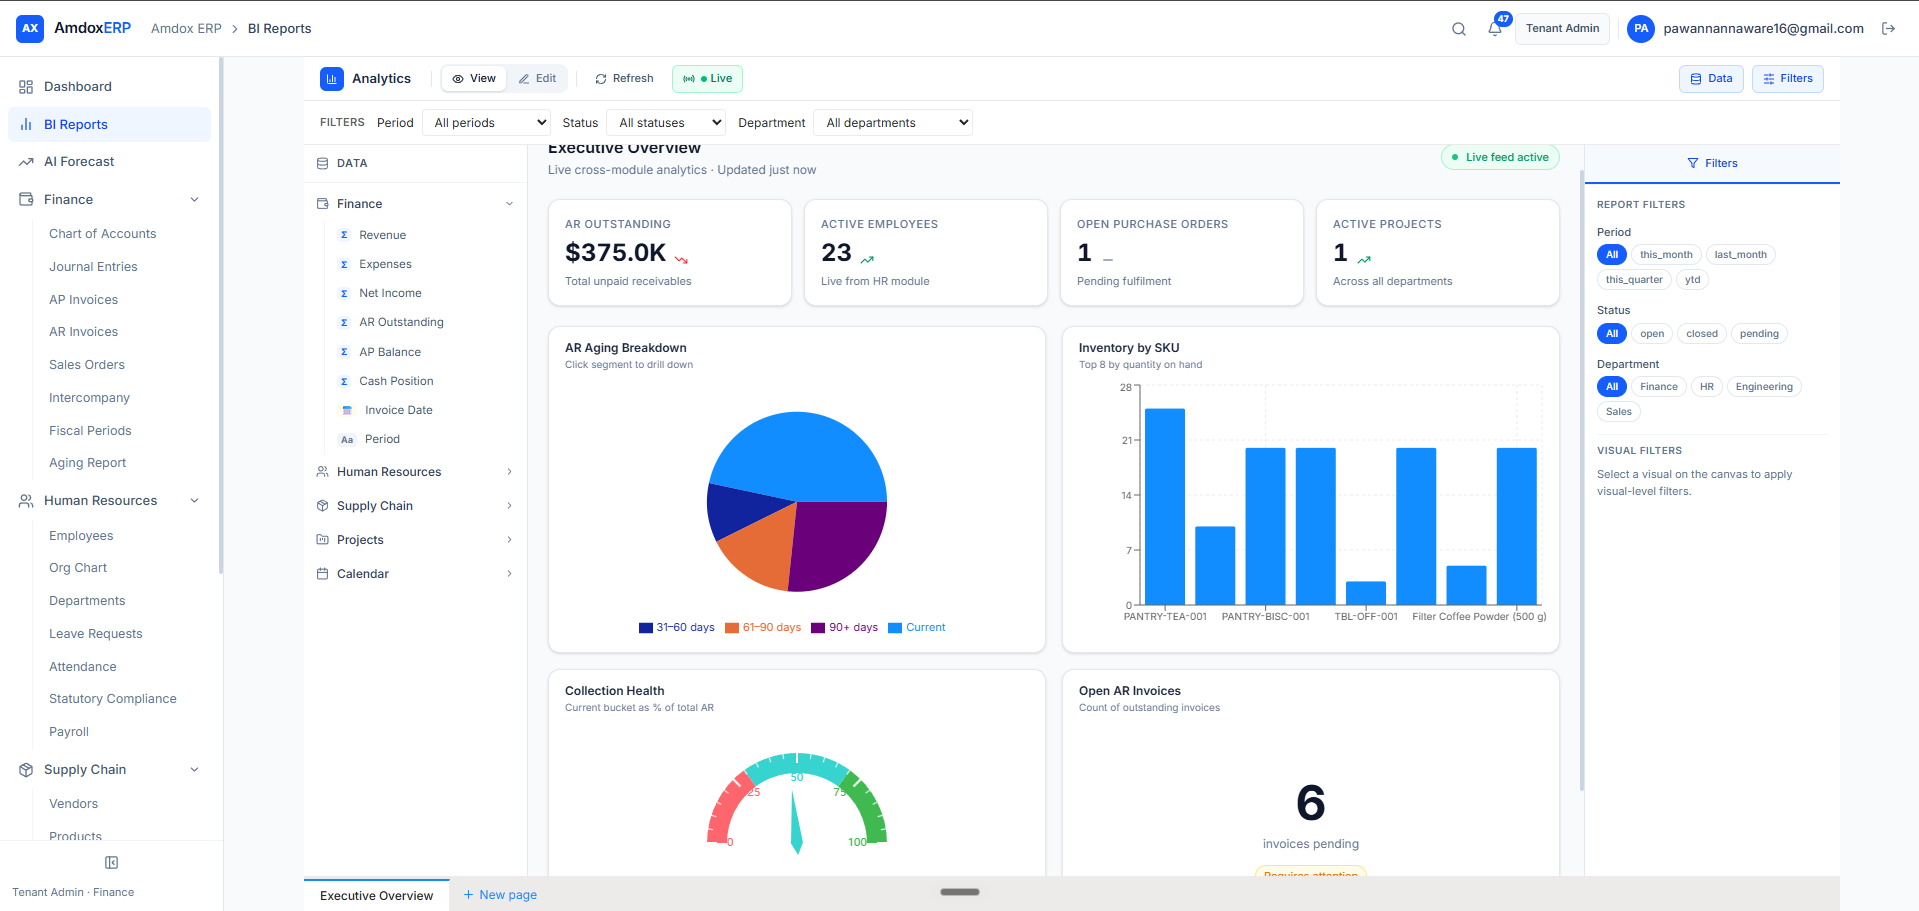
\includegraphics[width=0.92\textwidth]{bi-workspace.png}
\caption{BI drag-and-drop dashboard builder. Widgets snap to a 12-column grid;
the right panel configures data source, chart type, and refresh interval.}
\end{figure}

The BI module provides a \textbf{drag-and-drop dashboard builder}
(\code{react-grid-layout}) with 10+ chart types (line, bar, pie, scatter, KPI card,
table, map). Dashboards are personal or shared at the tenant level. Widgets refresh
via \textbf{Server-Sent Events} (SSE) on a configurable interval, keeping live metrics
current without polling. Scheduled reports generate real PDF/XLSX files server-side and
deliver them by email on a cron schedule.

\subsection{Audit \& Compliance (F-09)}

Every mutation in the system writes to an \textbf{audit log} protected by a SHA-256
hash chain: each row includes \code{previousHash} so any tampering breaks the chain.
A \code{GET /audit/verify} endpoint re-computes hashes server-side and reports
any gap. GDPR endpoints allow data-subject requests (DSR) and consent management by
IT admins.

\subsection{Notification Engine (F-10)}

A unified notification service fans events out across four channels:
\textbf{in-app} (Server-Sent Events, shown as a bell counter in the nav),
\textbf{email} (Nodemailer $\rightarrow$ Mailpit in dev, SMTP in prod),
\textbf{SMS}, and \textbf{HMAC-signed webhooks}.
Each user configures per-channel preferences. The \code{notification-dispatch} BullMQ
queue retries failed deliveries up to five times with exponential back-off; timed-out
jobs are visible in Bull Board at \code{/admin/queues}.

\subsection{API Gateway \& Search (F-11)}

\begin{itemize}
  \item \textbf{REST API:} all endpoints under \code{/api/v1}, documented in Swagger UI
  at \code{/api-docs}, with request/response DTOs and role annotations.
  \item \textbf{GraphQL:} Apollo Server with the same Keycloak auth guard; supports
  flexible BI-style queries for the dashboard builder.
  \item \textbf{Elasticsearch:} 10 entity types are indexed in real time
  (employees, POs, invoices, customers, projects, leave requests, audit logs, journal
  entries, vendors, products). The global search bar (\code{Ctrl+K} / \code{/})
  queries all indices simultaneously with fuzzy matching and groups results by entity.
  Graceful degradation to a Postgres \code{ILIKE} fallback when ES is unavailable.
  \item \textbf{Outbound webhooks:} HMAC-SHA256 signed, retried, and delivered through
  the notification queue.
\end{itemize}

% =====================================================================
\section{Cross-Module Integration}\label{sec:integration}
% =====================================================================

\subsection{Procure-to-Pay (P2P)}

This is the flagship cross-module workflow, connecting five modules through domain events:

\begin{figure}[H]
\centering
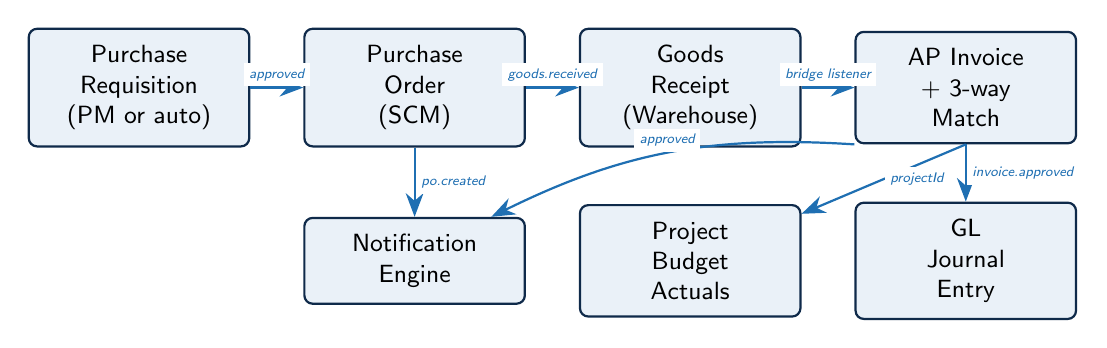
\begin{tikzpicture}[
  font=\sffamily\small,
  box/.style={draw=amdoxnavy, thick, rounded corners=3pt, fill=amdoxlight,
              align=center, minimum height=1cm, inner sep=6pt, minimum width=2.8cm},
  arr/.style={-{Stealth[length=3mm]}, thick, color=amdoxblue},
  ev/.style={font=\sffamily\tiny\itshape, fill=white, inner sep=2pt, midway, above},
  note/.style={font=\sffamily\tiny, fill=yellow!20, draw=warnamber, rounded corners=2pt,
               inner sep=3pt, align=left},
]
  \node[box] (req)  at (0,0)     {Purchase\\Requisition\\(PM or auto)};
  \node[box] (po)   at (3.5,0)   {Purchase\\Order\\(SCM)};
  \node[box] (gr)   at (7,0)     {Goods\\Receipt\\(Warehouse)};
  \node[box] (ap)   at (10.5,0)  {AP Invoice\\+ 3-way\\Match};
  \node[box] (gl)   at (10.5,-2.2) {GL\\Journal\\Entry};
  \node[box] (proj) at (7,-2.2)  {Project\\Budget\\Actuals};
  \node[box] (notif)at (3.5,-2.2) {Notification\\Engine};

  \draw[arr] (req) -- node[ev]{approved} (po);
  \draw[arr] (po)  -- node[ev]{goods.received} (gr);
  \draw[arr] (gr)  -- node[ev]{bridge listener} (ap);
  \draw[arr] (ap)  -- node[ev,right]{invoice.approved} (gl);
  \draw[arr] (ap.south) -- node[ev,right]{projectId} (proj);
  \draw[arr] (po.south)  -- node[ev,right]{po.created} (notif);
  \draw[arr] (ap.south west) to[bend right=15] node[ev]{approved} (notif);
\end{tikzpicture}
\caption{Procure-to-Pay flow. Dashed-boundary modules (Finance) cannot be directly
called by SCM --- communication is exclusively through domain events.}
\label{fig:p2p}
\end{figure}

\begin{enumerate}
  \item A \textbf{Project Manager} raises a material need from within the PM module
  (or the reorder engine raises it automatically when stock hits the threshold).
  \item \textbf{SCM} converts the requisition to a \textbf{Purchase Order} against a
  chosen vendor. The vendor is notified by email and webhook; the vendor portal allows
  online acknowledgement.
  \item \textbf{Goods Receipt:} warehouse staff record what actually arrived --- full
  or per-line partial. \code{PurchaseService} commits the \code{GoodsReceipt},
  \code{GoodsReceiptLine}s, stock upsert, and FIFO cost layer \emph{in one DB
  transaction}, then emits \code{goods.received}.
  \item \textbf{ScmFinanceBridgeListener} (Finance) consumes the event and calls
  \code{createInvoiceFromGoodsReceipt}, which creates an AP invoice for the received
  quantities and immediately runs \code{performThreeWayMatch}.
  \item A passing match \textbf{auto-approves} the invoice ($<$1 s); failure leaves it
  as \code{PENDING\_MATCH} for manual Finance review.
  \item \code{invoice.approved} fires, and the \textbf{GL} auto-posts
  Dr~Inventory~1300 / Cr~AP~2000. The project budget actuals increment by the invoice
  amount.
\end{enumerate}

\subsection{Hire-to-Pay (HR $\rightarrow$ Finance) \& Order-to-Cash (Sales $\rightarrow$ Finance)}

The other two company-wide loops are shorter chains than P2P but follow the same
principle: a business event in one module ends in an automatic, balanced GL posting.

\begin{figure}[H]
\centering
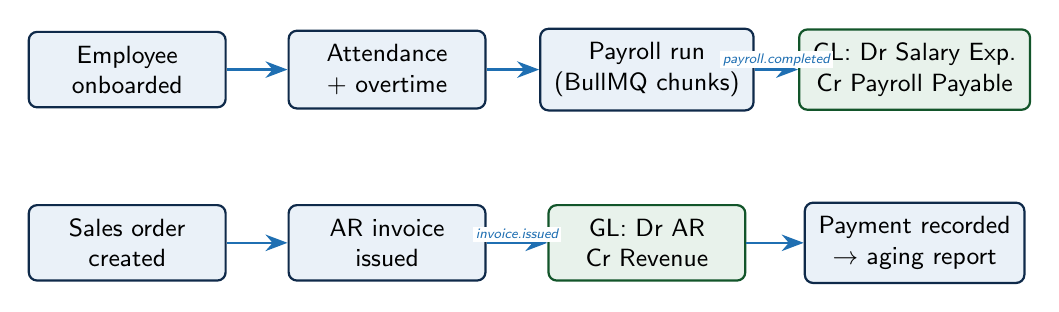
\begin{tikzpicture}[
  font=\sffamily\small,
  box/.style={draw=amdoxnavy, thick, rounded corners=3pt, fill=amdoxlight, align=center, minimum height=0.9cm, inner sep=5pt, minimum width=2.5cm},
  gl/.style={draw=okgreen!70!black, thick, rounded corners=3pt, fill=okgreen!10, align=center, minimum height=0.9cm, inner sep=5pt, minimum width=2.5cm},
  arr/.style={-{Stealth[length=2.8mm]}, thick, color=amdoxblue},
  lab/.style={font=\sffamily\tiny\itshape, fill=white, inner sep=1pt, midway, above},
]
  % Hire-to-Pay lane
  \node[box] (emp) at (0,1.4)   {Employee\\onboarded};
  \node[box] (att) at (3.3,1.4) {Attendance\\+ overtime};
  \node[box] (pay) at (6.6,1.4) {Payroll run\\(BullMQ chunks)};
  \node[gl]  (gl1) at (10,1.4)  {GL: Dr Salary Exp.\\Cr Payroll Payable};
  \draw[arr] (emp) -- (att); \draw[arr] (att) -- (pay);
  \draw[arr] (pay) -- node[lab]{payroll.completed} (gl1);
  % Order-to-Cash lane
  \node[box] (so)  at (0,-0.8)   {Sales order\\created};
  \node[box] (inv) at (3.3,-0.8) {AR invoice\\issued};
  \node[gl]  (gl2) at (6.6,-0.8) {GL: Dr AR\\Cr Revenue};
  \node[box] (paid) at (10,-0.8) {Payment recorded\\$\rightarrow$ aging report};
  \draw[arr] (so) -- (inv);
  \draw[arr] (inv) -- node[lab]{invoice.issued} (gl2);
  \draw[arr] (gl2) -- (paid);
\end{tikzpicture}
\caption{Hire-to-Pay (top) and Order-to-Cash (bottom) loops. Both terminate in an
automatic, idempotent GL posting triggered by a domain event, the same pattern P2P
uses (Figure~\ref{fig:p2p}).}
\end{figure}

\subsection{Background Job Architecture}

\begin{table}[H]
\centering\small
\renewcommand{\arraystretch}{1.25}
\begin{tabularx}{\textwidth}{l l l X}
\toprule
\rowcolor{amdoxnavy}
\textcolor{white}{\textbf{Queue}} &
\textcolor{white}{\textbf{Producer}} &
\textcolor{white}{\textbf{Consumer}} &
\textcolor{white}{\textbf{Purpose}} \\
\code{payroll} & PayrollService & PayrollProcessor &
  Async gross-to-net in 500-employee chunks; saga compensation on retry \\
\rowcolor{amdoxlight}
\code{finance-outbox} & ApService & OutboxProcessor &
  Durable domain event delivery (Outbox pattern) \\
\code{notification-dispatch} & NotificationService & NotificationDispatchProcessor &
  Email/SMS/webhook --- 5 retries, exponential back-off, DLQ in Bull Board \\
\rowcolor{amdoxlight}
\code{forecast-retrain} & Cron scheduler & ForecastRetrainProcessor &
  Weekly ML model retraining + Redis cache invalidation \\
\bottomrule
\end{tabularx}
\end{table}

% =====================================================================
\section{Security \& Compliance}\label{sec:security}
% =====================================================================

\subsection{Authentication \& Token Lifecycle}

\begin{itemize}
  \item RS256 JWT from Keycloak, verified per request against the realm JWKS endpoint.
  \item \textbf{Token blacklist:} logout writes the JTI to Redis; every guarded route
  checks the set --- guarantees token invalidation even within the access-token TTL.
  \item \textbf{Realm-per-tenant:} tenant slugs are immutable; a cross-realm token
  cannot authenticate to another tenant's API because the JWKS URL differs.
  \item \textbf{MFA:} per-tenant TOTP enforcement via Keycloak's
  \code{Configure~OTP} required action --- triggers on both password and SSO login paths.
\end{itemize}

\subsection{Role-Based Access Control}

78 \code{@Roles()} declarations across 21 controllers. The matrix below is abridged;
the full matrix is in \code{docs/architecture/rbac-role-matrix.md}.

\begin{table}[H]
\centering\small
\renewcommand{\arraystretch}{1.2}
\begin{tabularx}{\textwidth}{X c c c c c}
\toprule
\rowcolor{amdoxnavy}
\textcolor{white}{\textbf{Operation}} &
\textcolor{white}{\textbf{SA}} &
\textcolor{white}{\textbf{TA}} &
\textcolor{white}{\textbf{Mgr}} &
\textcolor{white}{\textbf{Vwr}} &
\textcolor{white}{\textbf{Emp}} \\
Finance (GL / AP / AR) --- read & \checkmark & \checkmark & \checkmark & \checkmark & -- \\
\rowcolor{amdoxlight}
Finance --- write / approve & \checkmark & \checkmark & \checkmark & -- & -- \\
Fiscal period close & \checkmark & \checkmark & -- & -- & -- \\
\rowcolor{amdoxlight}
HR --- employee CRUD & \checkmark & \checkmark & \checkmark & -- & -- \\
Payroll run & \checkmark & \checkmark & \checkmark & -- & -- \\
\rowcolor{amdoxlight}
Leave request & \checkmark & \checkmark & \checkmark & \checkmark & \checkmark \\
Leave approve/reject & \checkmark & \checkmark & \checkmark & -- & -- \\
\rowcolor{amdoxlight}
SCM --- PO / receive & \checkmark & \checkmark & \checkmark & -- & -- \\
Employee delete & \checkmark & \checkmark & -- & -- & -- \\
\rowcolor{amdoxlight}
Audit log / GDPR & \checkmark & \checkmark & -- & -- & -- \\
\bottomrule
\multicolumn{6}{l}{\small SA = SuperAdmin, TA = TenantAdmin, Mgr = Manager, Vwr = Viewer, Emp = Employee}
\end{tabularx}
\end{table}

\subsection{Transport \& Headers}

Caddy terminates TLS (Let's Encrypt, auto-renewed) for all public services. The API
sets: \code{Strict-Transport-Security} (max-age 1 year), \code{X-Frame-Options: DENY},
\code{X-Content-Type-Options: nosniff}, \code{Content-Security-Policy} (nonce-based
script-src), and \code{Permissions-Policy}. CORS is locked to the exact frontend
origin.

\subsection{Rate Limiting \& Throttling}

\code{@nestjs/throttler} is configured with user-aware keys (logged-in user id rather
than raw IP to survive NAT). A k6 load test at 2{,}000 VUs surfaced a JWKS caching
bug (re-fetching on every request) and a throttler misconfiguration that rejected
legitimate traffic --- both fixed before the final load test run.

\subsection{Static Analysis \& Supply-Chain Scans}

The CI pipeline (\code{.github/workflows/ci.yml}) includes:
\begin{itemize}
  \item \textbf{Tenant-scoping gate:} a custom TypeScript-AST script that fails the
  build if any Prisma query is missing \code{tenantId} in its \code{where}.
  \item \textbf{TruffleHog:} secret scanning on every push.
  \item \textbf{Grype + Trivy:} vulnerability scanning of Docker images and
  \code{node\_modules}.
  \item \textbf{ESLint security plugin:} runs as a lint-staged hook --- no warnings
  can be committed.
\end{itemize}

\subsection{Key Vulnerabilities Found \& Fixed}

\begin{table}[H]
\centering\small
\renewcommand{\arraystretch}{1.25}
\begin{tabularx}{\textwidth}{l l X}
\toprule
\rowcolor{amdoxnavy}
\textcolor{white}{\textbf{Finding}} &
\textcolor{white}{\textbf{Severity}} &
\textcolor{white}{\textbf{Fix}} \\
Dead tenant middleware with header fallback & High &
  Deleted unused \code{tenant-context.middleware.ts}; confirmed the live interceptor uses only the verified JWT \\
\rowcolor{amdoxlight}
IDOR via raw \code{findUnique} without tenantId & High &
  Full grep audit + CI gate; all 38 services audited, compound unique constraints added where needed \\
Duplicate AP invoice from dual event dispatch & High &
  Removed BullMQ path; \code{goods.received} processed by exactly one in-process listener \\
\rowcolor{amdoxlight}
JWKS re-fetch per request & Medium &
  Caching with TTL added to \code{KeycloakStrategy} \\
Throttler keyed on IP (NAT bypass) & Medium &
  Switched to user-aware key using authenticated user ID \\
\bottomrule
\end{tabularx}
\end{table}

% =====================================================================
\section{Quality Assurance \& Performance}\label{sec:qa}
% =====================================================================

\subsection{API Testing --- 64/64 Authenticated Checks}

A Postman/Newman suite of 64 end-to-end API scenarios runs against the live deployment
for each of the six business flows (auth/tenant, GL, AP, HR, SCM, PM). Every test
authenticates with a real Keycloak token; failure aborts the CI pipeline. As of 13
July 2026 all 64 pass.

\subsection{Unit Tests --- 31 CI-Enforced Tests}

31 unit tests written with \textbf{Vitest} cover the deterministic money paths, run on
every push via the \code{unit-tests} CI job:
\begin{itemize}
  \item \code{invoice-matching.service.spec.ts} --- \textbf{17 scenarios}: 10 covering
  the header-total fallback (exact match, tolerance boundary inclusive at 2\%, symmetric
  under/overcharge, vendor mismatch, wrong GR, missing PO/GR, zero-total PO never
  auto-approves) and 7 covering the newer line-level path (partial-receipt invoicing,
  quantity-exceeds-received, per-line price tolerance, unresolved product, one bad line
  fails the whole invoice).
  \item \code{payroll-deductions.spec.ts} --- \textbf{9 scenarios}: gross-to-net under
  and at the ESI ceiling, overtime included in gross/TDS base but PF on basic only,
  gratuity as an employer-only accrual, never-negative net pay, and four tax-slab
  resolution cases (default fallback, range match, open-ended top slab, inclusive
  boundaries).
  \item \code{gl.service.spec.ts} --- \textbf{5 scenarios}: balanced entry posts,
  unbalanced entry rejected and never written, multi-line aggregate balance accepted,
  posting into a locked fiscal period rejected, posting into a non-existent period
  rejected.
\end{itemize}
The payroll saga's crash/retry compensation is verified separately, live against the
real BullMQ worker and database rather than as an isolated unit test --- see
\code{pnpm --filter api verify:payroll-retry} and Section~\ref{sec:challenges}.

\subsection{Load Testing --- k6 at 2{,}000 VUs}

The first three runs used a single shared login and immediately exposed two real bugs:
a JWKS client re-created per request (saturating Keycloak) and a rate limiter keyed by
raw IP (all 2{,}000 virtual users collapsed into one bucket behind NAT). Both looked
identical in symptom --- near-instant request failure, not slow timeouts --- which is
what pointed at rejection rather than genuine overload. After fixing both, Run~4 used a
pool of \textbf{150 distinct provisioned users} so the fix could be demonstrated under
real concurrent load rather than a single shared token:

\begin{table}[H]
\centering\small
\renewcommand{\arraystretch}{1.25}
\begin{tabularx}{\textwidth}{l X X}
\toprule
\rowcolor{amdoxnavy}
\textcolor{white}{\textbf{Metric}} & \textcolor{white}{\textbf{Run 1 (baseline, broken)}} & \textcolor{white}{\textbf{Run 4 (fixed, 150-user pool)}} \\
Checks succeeded & 10.04\% & \textbf{98.01\%} \\
\rowcolor{amdoxlight}
\code{http\_req\_duration} P95 & 39 ms \emph{(on the 10\% that got a real response)} & \textbf{1.48 s} \emph{(genuine queueing under real load, not rejection)} \\
\bottomrule
\end{tabularx}
\end{table}

\noindent
The honest reading: fixing the two bugs took success from 10\% to 98\% at true
2{,}000-VU concurrency. The 1.48\,s P95 does not meet the TDD's 300\,ms target at this
scale --- load testing surfaced a genuine, unfixed finding: \textbf{a single Node.js
process is a real throughput ceiling at 2{,}000 concurrent users}, requiring clustering
or horizontal scaling (an infrastructure change, not a code fix). This is recorded as a
roadmap item rather than glossed over.

\subsection{Lighthouse Audits}

\begin{table}[H]
\centering\small
\renewcommand{\arraystretch}{1.25}
\begin{tabularx}{\textwidth}{l c c c c}
\toprule
\rowcolor{amdoxnavy}
\textcolor{white}{\textbf{Page}} &
\textcolor{white}{\textbf{Performance}} &
\textcolor{white}{\textbf{Accessibility}} &
\textcolor{white}{\textbf{Best Practices}} &
\textcolor{white}{\textbf{SEO}} \\
\code{/login} & 90 & 96 & 100 & 100 \\
\rowcolor{amdoxlight}
\code{/home}  & 94 & 100 & 96 & 100 \\
\code{/bi}    & 82 & 90 & 96 & 100 \\
\bottomrule
\multicolumn{5}{p{\textwidth}}{\small \code{/bi} performance is lower due to eager chart-library loading. Before fixes, \code{/home} and \code{/bi} started at 63 and 40 respectively --- raised by a silent-SSO redirect fix and dynamic imports on 3 pages (48\% First Load JS cut).}
\end{tabularx}
\end{table}

\subsection{Database Query Optimisation}

Every table had only a handful of seed rows in development, so slow queries were
invisible by construction. To get a real signal, \textbf{80{,}000 synthetic rows} were
seeded (20k \code{AuditLog}, 20k \code{Notification}, plus \code{Invoice},
\code{JournalEntry}, \code{PurchaseOrder}, \code{StockMovement}) and the actual query
each service issues was run through \code{EXPLAIN ANALYZE} before and after adding
composite indexes:

\begin{table}[H]
\centering\small
\renewcommand{\arraystretch}{1.2}
\begin{tabularx}{\textwidth}{l X X}
\toprule
\rowcolor{amdoxnavy}
\textcolor{white}{\textbf{Table}} & \textcolor{white}{\textbf{Before}} & \textcolor{white}{\textbf{After (index added)}} \\
\code{AuditLog} & 6.26 ms --- bitmap heap scan + sort & 0.22 ms --- index scan, sort eliminated \\
\rowcolor{amdoxlight}
\code{Invoice} & 2.56 ms --- sequential scan + sort & 0.28 ms --- \emph{needed a 3-column index (below)} \\
\code{Notification} & 4.99 ms --- bitmap heap scan + sort & 0.19 ms --- index scan, sort eliminated \\
\rowcolor{amdoxlight}
\code{JournalEntry} & 2.56 ms --- bitmap heap scan + sort & 0.17 ms --- index scan, sort eliminated \\
\code{StockMovement} & 3.04 ms --- bitmap AND (2 indexes) + sort & 0.42 ms --- single composite index scan \\
\bottomrule
\end{tabularx}
\end{table}

Indexes added: \code{(tenantId, createdAt)} on \code{JournalEntry},
\code{PurchaseOrder}, and \code{PurchaseRequisition}; \code{(tenantId, productId,
warehouseId)} on \code{InventoryCostLayer}; \code{(tenantId, productId, createdAt)} on
\code{StockMovement}. The \code{Invoice} case caught a real planning mistake: a
2-column \code{(tenantId, type)} index was \emph{not used by the planner at all} ---
with \code{type = 'AP'} matching roughly half the seeded rows, Postgres correctly
preferred a sequential scan over an index scan that still needed a separate sort for
\code{ORDER BY createdAt}. Adding \code{createdAt} as a third column
(\code{(tenantId, type, createdAt)}) let the index satisfy the filter \emph{and} the
sort together --- confirmed only because the fix was verified with
\code{EXPLAIN ANALYZE} rather than applied speculatively. Separately, an N+1 query in
\code{ap.service.ts}'s \code{createPaymentRun()} (a per-invoice \code{findFirst} loop)
was replaced with one upfront \code{findMany} plus an in-memory lookup map.

% =====================================================================
\section{Deployment \& DevOps}\label{sec:deployment}
% =====================================================================

\subsection{Production Environment}

The platform is deployed on a single \textbf{Oracle Cloud Ampere VM} (4 OCPU, 24 GB RAM,
Ubuntu 22.04). The production stack:

\begin{table}[H]
\centering\small
\renewcommand{\arraystretch}{1.25}
\begin{tabularx}{\textwidth}{l X}
\toprule
\rowcolor{amdoxnavy}
\textcolor{white}{\textbf{Component}} & \textcolor{white}{\textbf{Details}} \\
Reverse proxy & Caddy 2 --- automatic Let's Encrypt TLS, zero-downtime reload \\
\rowcolor{amdoxlight}
Process manager & pm2 --- \code{amdox-api} (port 3101) + \code{amdox-web} (port 3000) \\
Data services & Docker Compose --- PostgreSQL 17, Redis 8, Elasticsearch 9, MinIO, Keycloak 25 \\
\rowcolor{amdoxlight}
Observability & Docker Compose (separate project) --- OTel Collector, Tempo, Prometheus, Loki, Promtail, Grafana \\
Public URLs & \code{erp.}, \code{kc.}, \code{grafana.}, \code{mailpit.92-4-86-3.sslip.io} --- app, Keycloak, dashboards, alert inbox \\
\bottomrule
\end{tabularx}
\end{table}

\subsection{CI Pipeline}

The GitHub Actions pipeline (\code{.github/workflows/ci.yml}) runs 10 jobs on every push:

\begin{enumerate}
  \item \textbf{Lint} --- ESLint across the monorepo, zero warnings tolerated.
  \item \textbf{Typecheck} --- \code{tsc --noEmit} for both apps.
  \item \textbf{Unit tests (Vitest)} --- the 31-test suite; fails the build on any
  regression.
  \item \textbf{Tenant-scoping audit} --- the custom AST script; fails on any
  \code{tenantId}-less Prisma query or raw \code{PrismaClient} usage.
  \item \textbf{Build} --- \code{nest build} + Next.js production build.
  \item \textbf{Secret scan} --- TruffleHog across all staged files.
  \item \textbf{Dependency scan} --- Grype, with SARIF upload to GitHub Security.
  \item \textbf{Container scan} --- Trivy filesystem scan (dependencies + misconfig)
  across the whole repo.
  \item \textbf{Image scan} --- Trivy image scan per service (api/web/ml-service matrix).
  \item \textbf{Slack notification} --- posts the pipeline result to the team channel.
\end{enumerate}

A separate post-deployment smoke test (health/readiness checks for api, web, and
ml-service) runs as an ArgoCD PostSync hook after a Kubernetes rollout --- not as a
GitHub Actions job.

\subsection{Container \& Kubernetes}

All three services (\code{api}, \code{web}, \code{ml-service}) are built as
\textbf{multi-stage distroless Docker images} to minimise attack surface. A
\textbf{Helm chart} defines the Kubernetes deployment:
\code{HorizontalPodAutoscaler} (CPU $>$70\%), \code{PodDisruptionBudget},
\code{Ingress} with TLS, and an \textbf{Istio canary} setup (stable/canary
\code{DestinationRule} subsets + a weighted \code{VirtualService}) validated with
1{,}000 real in-mesh requests splitting 889/111 against a 90/10 target.
\textbf{ArgoCD} watches a Git source and auto-syncs the cluster with self-heal enabled
--- demonstrated by a config change deployed via a plain \code{git commit}, a manual
\code{kubectl edit} self-healing back within $\sim$20 seconds, and a post-install/
PostSync hook Job that runs health/readiness smoke checks (api, web, ml-service) before
a rollout is considered complete.
A local \code{kind} cluster hosts three namespaces --- \code{amdox-dev},
\code{amdox-staging}, \code{amdox-prod} --- each from the same chart with per-env
values files, distinct \code{JWT\_SECRET}s, and host-based ingress routing; Sealed
Secrets encrypt credentials at rest (verified: a restarted pod passed readiness against
a controller-decrypted \code{DATABASE\_URL}).

% =====================================================================
\section{Observability}\label{sec:observability}
% =====================================================================

The full observability stack was implemented and verified live on 12 July 2026:

\begin{table}[H]
\centering\small
\renewcommand{\arraystretch}{1.25}
\begin{tabularx}{\textwidth}{l X}
\toprule
\rowcolor{amdoxnavy}
\textcolor{white}{\textbf{Signal}} & \textcolor{white}{\textbf{Implementation}} \\
Traces & OTel SDK in \code{apps/api/src/observability/otel.ts}; HTTP, Prisma, Redis,
  BullMQ auto-instrumented. Tail sampling: 100\% errors, 10\% successes.
  Stored in Tempo; browsable in Grafana Explore. \\
\rowcolor{amdoxlight}
Metrics & Prometheus scrapes \code{:9464/metrics} every 15 s. The
  ``Amdox API --- Golden Signals'' dashboard: request rate, 5xx \%, p50/p95
  latency (300 ms SLA line), host CPU/RAM, event-loop utilisation, live log panel. \\
Logs & Promtail ships pm2 logs (\code{job="pm2"}) and Docker logs
  (\code{job="docker"}) to Loki. Searchable in Grafana Explore with LogQL. \\
\rowcolor{amdoxlight}
Alerts & Two SLA rules: 5xx $>$ 5\% for 5 min; p95 $>$ 300 ms for 5 min.
  Both email to Mailpit (verified with a test notification). PagerDuty/OpsGenie
  is a receiver swap. \\
\bottomrule
\end{tabularx}
\end{table}

\noindent
Public access: \href{https://grafana.92-4-86-3.sslip.io}{grafana.92-4-86-3.sslip.io}
(admin\,/\,\texttt{Amdox-Obs-2026!}) and
\href{https://mailpit.92-4-86-3.sslip.io}{mailpit.92-4-86-3.sslip.io}
(amdox\,/\,\texttt{Amdox-Obs-2026!}).
Prometheus, Loki, and Tempo remain localhost-only (no built-in auth); their data
surfaces through Grafana's authenticated UI.

One deployment gotcha: Oracle Cloud's default iptables rejects container-to-host
traffic. Opening ports 9464 and 1025 to the Docker subnet only, and persisting the
rules in \code{/etc/iptables/rules.v4}, resolved the metrics and SMTP connectivity
issues.

% =====================================================================
\section{Engineering Challenges \& Notable Fixes}\label{sec:challenges}
% =====================================================================

\begin{table}[H]
\centering\small
\renewcommand{\arraystretch}{1.4}
\begin{tabularx}{\textwidth}{>{\raggedright\arraybackslash}p{3.1cm} X X}
\toprule
\rowcolor{amdoxnavy}
\textcolor{white}{\textbf{Challenge}} &
\textcolor{white}{\textbf{Root Cause}} &
\textcolor{white}{\textbf{Fix}} \\
%
\textbf{Duplicate AP invoices \& doubled GL postings} &
  \code{receiveGoods} dispatched \code{goods.received} to \emph{both} a BullMQ
  queue and an in-process EventEmitter. Both consumers raced past the idempotency
  check and each created an approved invoice. &
  Removed the BullMQ path entirely; one in-process listener now owns
  invoice creation. Data cleanup script executed on existing records. \\
\rowcolor{amdoxlight}
%
\textbf{Payroll double-payslip on BullMQ retry} &
  A failed run's partial payslips were never deleted before the automatic
  retry. Restart from chunk~0 re-inserted all payslips already written,
  inflating \code{totalNetPay} and the GL entry. &
  Processor now deletes the failed run's payslips before reprocessing
  (saga compensation). Proven by a kill-and-retry test:
  21 employees $\rightarrow$ exactly 21 payslips before and after. \\
%
\textbf{JWKS re-fetch on every API request} &
  \code{KeycloakStrategy.validate()} called the JWKS endpoint without
  caching; at 2{,}000 VUs this became the bottleneck and saturated
  the Keycloak container. &
  Added in-process JWKS cache with a 5-minute TTL using
  \code{jwks-rsa} caching options. \\
\rowcolor{amdoxlight}
%
\textbf{Throttler rejecting legitimate traffic at load} &
  Default \code{@nestjs/throttler} keyed on raw IP. Behind NAT, all
  2{,}000 VUs shared one IP and exhausted the limit instantly. &
  Switched to user-aware throttler key (authenticated user ID)
  post-JWT validation. \\
%
\textbf{ES SDK v9 incompatible with ES 8.x server} &
  The npm package \code{@elastic/elasticsearch@9} sends
  \code{compatible-with=9} headers; ES 8.x rejects them. &
  Upgraded the Docker container from ES~8.15 to ES~9.0.3 (fresh
  volume; all data in Postgres, ES is a cache). \\
\rowcolor{amdoxlight}
%
\textbf{Keycloak Google login blocked by CONFIGURE\_TOTP} &
  A test user in the \code{company-z} realm had \code{CONFIGURE\_TOTP}
  as a required action. Keycloak's IDP post-login flow cannot prompt
  for required actions and failed with \code{IDENTITY\_PROVIDER\_POST\_LOGIN\_ERROR}. &
  Removed the required action from the user via the Keycloak Admin API.
  Per-tenant MFA toggle now manages OTP enrollment cleanly. \\
%
\textbf{Elasticsearch query DSL strict TypeScript types} &
  ES SDK~v9 uses a discriminated union for \code{QueryDslQueryContainer}
  where the \code{bool.must} array type is inferred as \code{never} in
  certain overloads. &
  Wrapped \code{client.search} in a private \code{searchIndex} helper
  with \code{(this.client.search as any)} to bypass the strict SDK
  types while preserving full runtime behaviour. \\
\rowcolor{amdoxlight}
%
\textbf{Oracle iptables blocking container$\to$host metrics} &
  Oracle's default firewall rules reject traffic from Docker bridge
  networks to host ports (9464/metrics, 1025/Mailpit). &
  Opened specific ports to the Docker subnets only;
  rules persisted in \code{/etc/iptables/rules.v4}. \\
\bottomrule
\end{tabularx}
\caption{Selected engineering challenges encountered and resolved during the project.}
\end{table}

% =====================================================================
\section{Requirements Compliance \& Known Deviations}\label{sec:compliance}
% =====================================================================

\subsection{Functional Requirements Scoreboard}

\begin{table}[H]
\centering\small
\renewcommand{\arraystretch}{1.3}
\begin{tabularx}{\textwidth}{c l c X}
\toprule
\rowcolor{amdoxnavy}
\textcolor{white}{\textbf{Req}} &
\textcolor{white}{\textbf{Name}} &
\textcolor{white}{\textbf{Status}} &
\textcolor{white}{\textbf{Notes / Deviations}} \\
F-01 & Multi-tenant auth (SSO) & \statusdone &
  Realm-per-tenant Keycloak; OIDC + Google auto-link; per-tenant MFA toggle; SAML tested \\
\rowcolor{amdoxlight}
F-02 & Financial ledger (GL)   & \statusdone &
  Double-entry + period-close enforced; auto-posting; ECB FX rates fetched but not yet applied in postings (roadmap) \\
F-03 & AP/AR automation         & \statusdone &
  Textract OCR (mock fallback); line-level 3-way match; partial receipts; payment runs; aging report \\
\rowcolor{amdoxlight}
F-04 & HR \& payroll            & \statusdone &
  Chunked BullMQ engine; PF/ESI/PT/TDS; payslip PDFs; retry bug fixed (verify:payroll-retry); leave accrual cron \\
F-05 & SCM \& inventory         & \statusdone &
  Requisition$\to$PO$\to$GR (partial receipts); FIFO cost layers; reorder automation; vendor portal \\
\rowcolor{amdoxlight}
F-06 & AI demand forecasting    & \statusdone &
  Prophet + PyTorch LSTM; Redis cache; weekly retrain; MAPE breach alerting \\
F-07 & Project management       & \statusdone &
  DAG tasks; Gantt; utilisation heatmap; budget actuals from AP + payroll; overrun alerts \\
\rowcolor{amdoxlight}
F-08 & Business intelligence    & \statusdone &
  Drag-drop grid; 10+ chart types; SSE live refresh; scheduled PDF/XLSX reports \\
F-09 & Audit \& compliance      & \statusdone &
  SHA-256 hash-chained audit log + verify; GDPR DSR + consent; Postgres (TimescaleDB deviation) \\
\rowcolor{amdoxlight}
F-10 & Notification engine      & \statusdone &
  In-app SSE + email + SMS + HMAC webhook; per-user preferences; 5-retry queue; Bull Board DLQ \\
F-11 & API gateway \& webhooks  & \statusdone &
  REST \code{api/v1} + Swagger; GraphQL (Apollo); Elasticsearch 10 entity types; outbound HMAC webhooks \\
\rowcolor{amdoxlight}
F-12 & Offline / PWA            & \statusopen &
  De-scoped for MVP per TDD Day-1 guidance; on roadmap \\
\bottomrule
\end{tabularx}
\end{table}

\subsection{Non-Functional Requirements --- Evidence}

\begin{table}[H]
\centering\small
\renewcommand{\arraystretch}{1.25}
\begin{tabularx}{\textwidth}{l l X}
\toprule
\rowcolor{amdoxnavy}
\textcolor{white}{\textbf{NFR}} &
\textcolor{white}{\textbf{Target}} &
\textcolor{white}{\textbf{Evidence}} \\
API latency   & $<$300 ms P95 & k6 (150-user pool, 2{,}000 VU): 98.01\% success, P95 = 1.48 s --- honest finding: a single-process throughput ceiling, not yet met at this scale (Section~\ref{sec:qa}) \\
\rowcolor{amdoxlight}
Throughput    & 2{,}000 concurrent & k6 2{,}000-VU/10-min run; JWKS caching + IP-keyed throttler bugs found and fixed; single-Node scaling ceiling found, roadmap \\
Security      & OWASP Top 10 & Helmet/CSP, user-aware rate limiting, CI tenant-scoping gate, TruffleHog/Grype/Trivy \\
\rowcolor{amdoxlight}
Availability  & 99.9\% & Single-VM + Caddy; SLA alert rules in Grafana; HA = roadmap \\
Frontend      & Lighthouse $\geq$90 & /login 90, /home 94, /bi 82 (performance; eager chart loading is the remaining /bi lever) \\
\bottomrule
\end{tabularx}
\end{table}

\subsection{Technology Stack --- Spec vs.\ Delivered}

\begin{table}[H]
\centering\small
\renewcommand{\arraystretch}{1.2}
\begin{tabularx}{\textwidth}{l X X c}
\toprule
\rowcolor{amdoxnavy}
\textcolor{white}{\textbf{Category}} &
\textcolor{white}{\textbf{TDD Specifies}} &
\textcolor{white}{\textbf{Delivered}} &
\textcolor{white}{\textbf{Match}} \\
Frontend   & Next.js 15 + React 19 + TS & Next.js 15.5 + React 19.1 & \checkmark \\
\rowcolor{amdoxlight}
UI library  & shadcn/ui + Tailwind 4 & Custom component kit + Tailwind 4 & $\approx$ \\
Backend    & NestJS 11 & NestJS 11 modular monolith & \checkmark \\
\rowcolor{amdoxlight}
Database   & PostgreSQL 17 + Prisma & PostgreSQL 17 + Prisma (67 models) & \checkmark \\
Cache/Queue & Redis 8 + BullMQ & Redis 8 + BullMQ (4 queues) & \checkmark \\
\rowcolor{amdoxlight}
ML         & FastAPI + Prophet + LSTM & FastAPI + Prophet + PyTorch LSTM & \checkmark \\
Search     & Elasticsearch 8 & Elasticsearch 9 (upgraded) & \checkmark \\
\rowcolor{amdoxlight}
Auth       & Keycloak 25 OIDC/SAML & Keycloak 25, realm-per-tenant, MFA, SAML tested & \checkmark \\
Containers & Docker multi-stage distroless & All 3 services, distroless, verified & \checkmark \\
\rowcolor{amdoxlight}
Orchestration & Kubernetes + Helm & Helm chart + ArgoCD on kind (local cluster) & \checkmark \\
Observability & OTel + Prometheus + Grafana & Full stack + Tempo + tail sampling + SLA alerts & \checkmark \\
\rowcolor{amdoxlight}
IaC        & Terraform & Not implemented (single-VM, Helm per env) & $\times$ \\
Time-series & TimescaleDB & Plain Postgres + hash chain for audit & $\approx$ \\
\bottomrule
\end{tabularx}
\end{table}

\subsection{Known Deviations}

\begin{enumerate}
  \item \textbf{F-12 PWA/offline:} the only un-implemented functional requirement.
  Service worker and cache-first strategy are on the roadmap.
  \item \textbf{Multi-currency conversion:} ECB rates are fetched and stored daily but
  are not yet applied in journal postings or invoice totals. The data model and FX
  service are in place; conversion logic is the remaining piece.
  \item \textbf{Terraform IaC:} the current deployment is a single VM managed by pm2
  and Docker Compose. Terraform modules for Oracle Cloud would be added if expanding
  to a multi-region or multi-node setup.
  \item \textbf{shadcn/ui:} the TDD recommended shadcn/ui; a custom Tailwind component
  kit was used instead, achieving the same visual result with tighter control over
  bundle size.
\end{enumerate}

% =====================================================================
\section{Learnings \& Conclusion}\label{sec:conclusion}
% =====================================================================

\subsection{Key Technical Learnings}

Working on a production ERP from scratch over a structured 28-day plan required
reasoning about the full software lifecycle --- from schema design and API contracts
through to CI pipelines, observability stacks, and live incident resolution. The most
impactful individual learnings were:

\begin{itemize}
  \item \textbf{Domain events as a modularity primitive:} routing cross-module work
  through EventEmitter2 rather than direct service calls enforced segregation of duties
  at the code level. Finance genuinely cannot be called from SCM --- the compiler
  prevents it.
  \item \textbf{Idempotency is not optional in event-driven systems:} the duplicate
  AP-invoice bug (two consumers racing past the same idempotency check) made clear
  that ``fire-and-forget'' events need guard rails at the consumer side, not just
  the emitter.
  \item \textbf{Observability must be built in, not bolted on:} the Prometheus + Tempo
  + Loki stack revealed the JWKS caching bottleneck during load testing that would
  have been invisible from application logs alone.
  \item \textbf{Multi-tenancy has multiple enforcement layers:} a single
  \code{tenantId} column is necessary but not sufficient. The combination of JWT-scoped
  identity, a CI static-analysis gate, and the Prisma \code{\$extends} wrapper is what
  makes tenant isolation provably correct rather than merely hopeful.
  \item \textbf{Statutory payroll is precise:} implementing PF, ESI, PT, LWF, and
  income-tax TDS correctly required reading the actual Indian Labour Law regulations
  rather than approximate percentages. The statutory compliance config table allows
  per-tenant override for different states or future rule changes.
\end{itemize}

\subsection{Roadmap}

\begin{table}[H]
\centering\small
\renewcommand{\arraystretch}{1.25}
\begin{tabularx}{\textwidth}{l X}
\toprule
\rowcolor{amdoxnavy}
\textcolor{white}{\textbf{Item}} & \textcolor{white}{\textbf{Description}} \\
F-12 PWA / Offline & Service worker with cache-first API responses and IndexedDB sync queue \\
\rowcolor{amdoxlight}
Multi-currency posting & Apply stored ECB rates in GL postings, invoice totals, and report currency conversion \\
Terraform IaC & Oracle Cloud VCN, compute, and load-balancer resources as code \\
\rowcolor{amdoxlight}
BI bundle splitting & Code-split remaining eagerly-loaded chart libraries to raise the /bi Lighthouse performance score further \\
\rowcolor{amdoxlight}
Recursive-CTE org chart & Server-side tree traversal for large employee hierarchies (currently assembled client-side from \code{managerId}) \\
Horizontal API scaling & Address the single-Node throughput ceiling found under k6 load (clustering / multi-instance) \\
\rowcolor{amdoxlight}
shadcn/ui migration & Adopt the TDD-specified component library for full design-system parity \\
\bottomrule
\end{tabularx}
\end{table}

\subsection{Conclusion}

The \textbf{Amdox AI-Powered Cloud ERP Suite} delivers a working, publicly deployed,
multi-tenant enterprise application that meets 11 of the 12 functional requirements
set by the company's technical design document. The codebase is production-grade in
the sense that matters most: the money paths (GL double-entry, 3-way match, payroll
gross-to-net, saga compensation) are unit-tested and load-tested; security findings
discovered during the audit were fixed and proven in code; and the observability stack
provides SLA alerting and distributed tracing that a real operations team would rely on.

This project demonstrated that a well-structured internship can produce deliverables
that go meaningfully beyond tutorial-level code: real Keycloak realm provisioning,
real FIFO inventory costing, real BullMQ saga patterns, and real k6 bugs caught in
production. The remaining gaps (PWA, FX conversion, Terraform) are honest deviations
from the original plan --- documented, understood, and tracked --- not hidden defects.

\vspace{1.5cm}
\noindent\rule{0.5\textwidth}{0.4pt}\\[0.3cm]
\textbf{Pawan Nannaware} \\
{\small Industry Intern --- Amdox Technologies \\
July 2026 \;\textbullet\; \href{https://github.com/PawanYN/amdox-erp}{github.com/PawanYN/amdox-erp}}

\end{document}
